\documentclass[oneside,a4paper,11pt]{book} 
\setcounter{secnumdepth}{4}
\setcounter{tocdepth}{4}   
\usepackage{fancyhdr}
\setlength{\headheight}{15pt}
\usepackage[pdftex,
pdfauthor={Name, Vorname},
pdftitle={Überschrift},
pdfsubject={Projektarbeit},
pdfkeywords={Unterschrift}
]{hyperref}
\usepackage[ngerman]{babel}
\usepackage[T1]{fontenc}
\usepackage[utf8]{inputenc}
\usepackage[dvips]{graphicx}
\usepackage{calc}
\usepackage{makeidx}
\usepackage{xcolor}
\usepackage[hang,small,scriptsize,bf]{caption}
\usepackage{hsel-thesis2020}
\usepackage{amssymb}
\usepackage{amsmath}
\usepackage{subcaption}
\usepackage{hyperref}
\usepackage{multirow}
\usepackage{circuitikz}
\usepackage{seqsplit}
\usepackage{csquotes}
\usepackage{makecell}
\usepackage{animate}
\usepackage{eso-pic}
\usepackage{newfloat}
\usepackage{pdfpages}
\usepackage{tikz}
\usepackage{listings}
\usepackage{fixltx2e}
\usepackage{flowchart}
\usepackage[normalem]{ulem}
\usepackage[
  style=numeric,
  sorting=none,
  backend=biber
  ]{biblatex}
\addbibresource{Literaturverzeichnis.bib}
\usetikzlibrary{positioning}




\newcommand{\myboxy}[3]{
	\begin{tikzpicture}[
			every node/.style={rectangle,rounded corners,draw=black, top color=white,very thick, inner sep=0.3em, minimum size=1em} ]
		\node[text width=#3](main) at (0,0 ){\vspace{3pt}  #1};
		\node[above =-2mm of main.north west, anchor=south west] (title) {#2};
	\end{tikzpicture} }



\newcommand{\textbfit}[1]{\textbf{\textit{#1}}}


\pdfcompresslevel=5 



\DeclareFloatingEnvironment[
	listname  = {Diagrammverzeichnis}, % Listenüberschrift
	name      = Diagramm,              % Name in Beschriftungen
]{scheme}


\DeclareFloatingEnvironment[
	listname  = {Oszillogrammverzeichnis}, % Listenüberschrift
	name      = Oszillogramm,              % Name in Beschriftungen
]{oszillo}


%%%%%%%%%%%%%%%%%%%%%%%%%%%%%%%%%%%%%%%%%%%%%%%%%%%%%%%%%%%%%%%%%%%%%%%%%%%%%%%%%%%%
%%%%%%%%%%%%%%%%%%%%%%%%%%%%%%%%%%%%%%%%%%%%%%%%%%%%%%%%%%%%%%%%%%%%%%%%%%%%%%%%%%%%
%%%%%%%%%%%%%%%%%%%%%%%%%%%%%%%%%%%%%%%%%%%%%%%%%%%%%%%%%%%%%%%%%%%%%%%%%%%%%%%%%%%%
%%%%%%%%%%%%%%%%%%%%%%%%%%%%%%%%%%%%%%%%%%%%%%%%%%%%%%%%%%%%%%%%%%%%%%%%%%%%%%%%%%%%
%%%%%%%%%%%%%%%%%%%%%%%%%%%%%%%%%%%%%%%%%%%%%%%%%%%%%%%%%%%%%%%%%%%%%%%%%%%%%%%%%%%%
%%%%%%%%%%%%%%%%%%%%%%%%%%%%%%%%%%%%%%%%%%%%%%%%%%%%%%%%%%%%%%%%%%%%%%%%%%%%%%%%%%%%


\begin{document}
\allsectionsfont{\sffamily}


\AddToShipoutPicture{\BackgroundWave}
\pagenumbering{Roman}

\include{source/0_0_Titelseite}
\linespread{1.2}
\noitemsep
\include{source/0_1_RechtlicheErklärung}
\include{source/0_2_Verzeichnis}

\cleardoublepage
\pagenumbering{arabic}
\ClearShipoutPicture

\chapter{Einleitung}
\label{chapter:Einleitung}

\section{Motivation der Hyperloop Technologie}
\label{section:Motivation}

Der Hyperloop ist ein innovatives Transportkonzept, das eine ökonomische, klimafreundliche und schnellere Alternative zu herkömmlichen Verkehrsmitteln wie Lastkraftwagen, Zügen und Flugzeugen bietet.\\
\pagebreak[3]
\begin{figure}[!ht]
	\begin{center}
		\includegraphics[width=1\textwidth]{img/1_strecke/strecke_1.png}
		\caption{Hyperloop der Hochschule Emden-Leer}
		\label{img_1_1:strecke}
	\end{center}
\end{figure}
\pagebreak[4]
Derzeit stehen herkömmlichen Transportmitteln zwei wesentliche Hindernisse im Weg, um Personen und Güter schnell und emissionsarm zu befördern. Zum einen der hohe Luftwiderstand, der bei hohen Geschwindigkeiten den Energieverbrauch stark erhöht.\\
Der Hyperloop löst diese Probleme, indem er Güter und Personen in einem Fahrzeug, das sich in einer fast Vakuumröhre bewegt, wie in Abbildung \ref{img_1_1:strecke} dargestellt ist.



%%%%%%%%%%%%%%%%%%%%%%%%%%%%%%%%%%%%%%%%%%%%%%%%%%%%%%%%%%%%%%%%%%%%%%%%%%%%%%%%%%%%
%%%%%%%%%%%%%%%%%%%%%%%%%%%%%%%%%%%%%%%%%%%%%%%%%%%%%%%%%%%%%%%%%%%%%%%%%%%%%%%%%%%%
%%%%%%%%%%%%%%%%%%%%%%%%%%%%%%%%%%%%%%%%%%%%%%%%%%%%%%%%%%%%%%%%%%%%%%%%%%%%%%%%%%%%
%%%%%%%%%%%%%%%%%%%%%%%%%%%%%%%%%%%%%%%%%%%%%%%%%%%%%%%%%%%%%%%%%%%%%%%%%%%%%%%%%%%%
%%%%%%%%%%%%%%%%%%%%%%%%%%%%%%%%%%%%%%%%%%%%%%%%%%%%%%%%%%%%%%%%%%%%%%%%%%%%%%%%%%%%
%%%%%%%%%%%%%%%%%%%%%%%%%%%%%%%%%%%%%%%%%%%%%%%%%%%%%%%%%%%%%%%%%%%%%%%%%%%%%%%%%%%%



\subsection*{Institute of Hyperloop Technology}
\label{section:IHT}

%Die Hochschule Emden/Leer hat im Jahr 2021 das Institut für Hyperloop-Technologie (IHT) gegründet, um aktiv an der Forschung zu dieser zukunftsweisenden Technologie teilzunehmen.

Im Rahmen dieser Forschung-arbeit, -projekt wurde an der Hochschule Emden eine Teststrecke mit einer Länge von 27 Metern errichtet (siehe Abbildung \ref{img_1_1:strecke}). Auf dieser Strecke soll das Fahrzeug (Cargo-Pod) unter realistischen Bedingungen getestet und weiterentwickelt werden.
Die Teststrecke besteht aus einem Schienensystem und einem Linearmotor.\\
Die Forschung des \frqq Institute of Hyperloop Technology\flqq, fokuziert sich auf die Güterbeförderung.
\newpage




\section{Aufgabenstellung}
\label{section:Aufgabenstellung}
Das Ziel dieses Projektes ist die Entwilckung eines Hyperloop-Fahrzeuges, das mit einer Batterie und einem Motor betrieben wird. Für die Steuerung des Fahrzeugs wurde ein echtzeitfähiges Steuerungsystem der Firma Speedgoat vorgeben, welches in Abschnitt \ref{section:speedgoat} vertiefend erläutert wird.\\ \ \\

Im Rahmen des Projekts wird ein Fahrzeug (Pod) für den Hyperloop mit einer Bordspannung von 48 V konzipiert. Ziel ist es, die Realisierbarkeit dieser Spannung zu überprüfen und umzusetzen. Dazu gehören die Planung und Simulierung, die Integration der erforderlichen Sensorik sowie die Beschaffung der notwendigen Bauteile. Die Logik- und Signalverarbeitung wird, mithilfe von Simulink, auf dem echtzeitfähigen Speedgoat-System durchgeführt.
Die Steuerung erfolgt über Simulink, ein Modul von MATLAB, und beinhaltet die Erfassung von Position und Beschleunigung des Fahrzeuges. Der Motor wird über ein zusätzliches Steuergerät angesteuert. Die Steuerung soll in Form einer Automatensteuerung umgesetzt werden.
Die Verdrahtung des Pods wird entsprechend der Bordspannung von 48 V ausgelegt. Hierfür wird mit der Software QElectroTech ein Schaltplan (siehe Anhang \ref{Anhang:Schaltplan}) erstellt.
Alle erforderlichen Bauteile für die Umsetzung der Bordspannung, die Verdrahtung und die Sensorik müssen beschafft werden.\\
Textergebnisse und Inbetriebnahme entfallen.


%%%%%%%%%%%%%%%%%%%%%%%%%%%%%%%%%%%%%%%%%%%%%%%%%%%%%%%%%%%%%%%%%%%%%%%%%%%%%%%%%%%%
%%%%%%%%%%%%%%%%%%%%%%%%%%%%%%%%%%%%%%%%%%%%%%%%%%%%%%%%%%%%%%%%%%%%%%%%%%%%%%%%%%%%
%%%%%%%%%%%%%%%%%%%%%%%%%%%%%%%%%%%%%%%%%%%%%%%%%%%%%%%%%%%%%%%%%%%%%%%%%%%%%%%%%%%%
%%%%%%%%%%%%%%%%%%%%%%%%%%%%%%%%%%%%%%%%%%%%%%%%%%%%%%%%%%%%%%%%%%%%%%%%%%%%%%%%%%%%
%%%%%%%%%%%%%%%%%%%%%%%%%%%%%%%%%%%%%%%%%%%%%%%%%%%%%%%%%%%%%%%%%%%%%%%%%%%%%%%%%%%%
%%%%%%%%%%%%%%%%%%%%%%%%%%%%%%%%%%%%%%%%%%%%%%%%%%%%%%%%%%%%%%%%%%%%%%%%%%%%%%%%%%%%

\section{Aufbau der Projektdokumentation}
\label{section:Aufbau}


Die Projektdokumentation beginnt mit einer Einführung in die Hyperloop-Technologie und der Aufgabenstellung dieses Projekts, die die Motivation und Zielsetzungen erläutern. Es wird dargelegt, warum der Hyperloop als innovative, umweltfreundliche Transportlösung eine wichtige Alternative zu bestehenden Systemen darstellt und welche spezifischen Herausforderungen und Ziele mit der Entwicklung eines funktionsfähigen Prototyps verbunden sind.

Im weiteren Verlauf wird das grundlegende Fahrzeugkonzept vorgestellt. Dabei wird beschrieben, wie die verschiedenen Baugruppen miteinander verbunden sind und welche Rolle das zentrale Steuerungssystem von Speedgoat übernimmt. Auch die verwendeten Sensoren und deren Einbindung in das Gesamtsystem werden erläutert.

Der Dokumentationsteil zur Implementierung zeigt die technische Realisierung der Steuerung und der elektrischen Verdrahtung des Fahrzeugs. Die Erstellung des Schaltplans, die Konfiguration der Steuerlogik sowie die detaillierte Beschreibung der Automatik- und manuellen Steuerungsmodi geben Einblicke in die Funktionsweise und den Aufbau des Systems. Ergänzend wird die Integration der Distanzmessung beschrieben, die eine präzise Positionsermittlung innerhalb der Teststrecke ermöglicht.

Abschließend fasst die Konklusion die Ergebnisse der Projektarbeit zusammen und gibt Hinweise auf mögliche zukünftige Entwicklungen. Hierbei wird auch die Offenheit der Systemarchitektur betont, die eine flexible Weiterentwicklung ermöglicht..


%%%%%%%%%%%%%%%%%%%%%%%%%%%%%%%%%%%%%%%%%%%%%%%%%%%%%%%%%%%%%%%%%%%%%%%%%%%%%%%%%%%%
%%%%%%%%%%%%%%%%%%%%%%%%%%%%%%%%%%%%%%%%%%%%%%%%%%%%%%%%%%%%%%%%%%%%%%%%%%%%%%%%%%%%
%%%%%%%%%%%%%%%%%%%%%%%%%%%%%%%%%%%%%%%%%%%%%%%%%%%%%%%%%%%%%%%%%%%%%%%%%%%%%%%%%%%%
%%%%%%%%%%%%%%%%%%%%%%%%%%%%%%%%%%%%%%%%%%%%%%%%%%%%%%%%%%%%%%%%%%%%%%%%%%%%%%%%%%%%
%%%%%%%%%%%%%%%%%%%%%%%%%%%%%%%%%%%%%%%%%%%%%%%%%%%%%%%%%%%%%%%%%%%%%%%%%%%%%%%%%%%%
%%%%%%%%%%%%%%%%%%%%%%%%%%%%%%%%%%%%%%%%%%%%%%%%%%%%%%%%%%%%%%%%%%%%%%%%%%%%%%%%%%%%
\include{source/einennoch}
\chapter{Konzept}
\label{chapter:Konzept}


Im Folgenden wird der Aufbau des Fahrzeugs erklärt und welche Sensoren verbaut werden. Dabei übernimmt das Steuerungs- und Datenerfassungskonzept von Speedgoat eine zentrale Rolle.\\
\pagebreak[1]
\begin{figure}[!ht]
	\begin{center}
		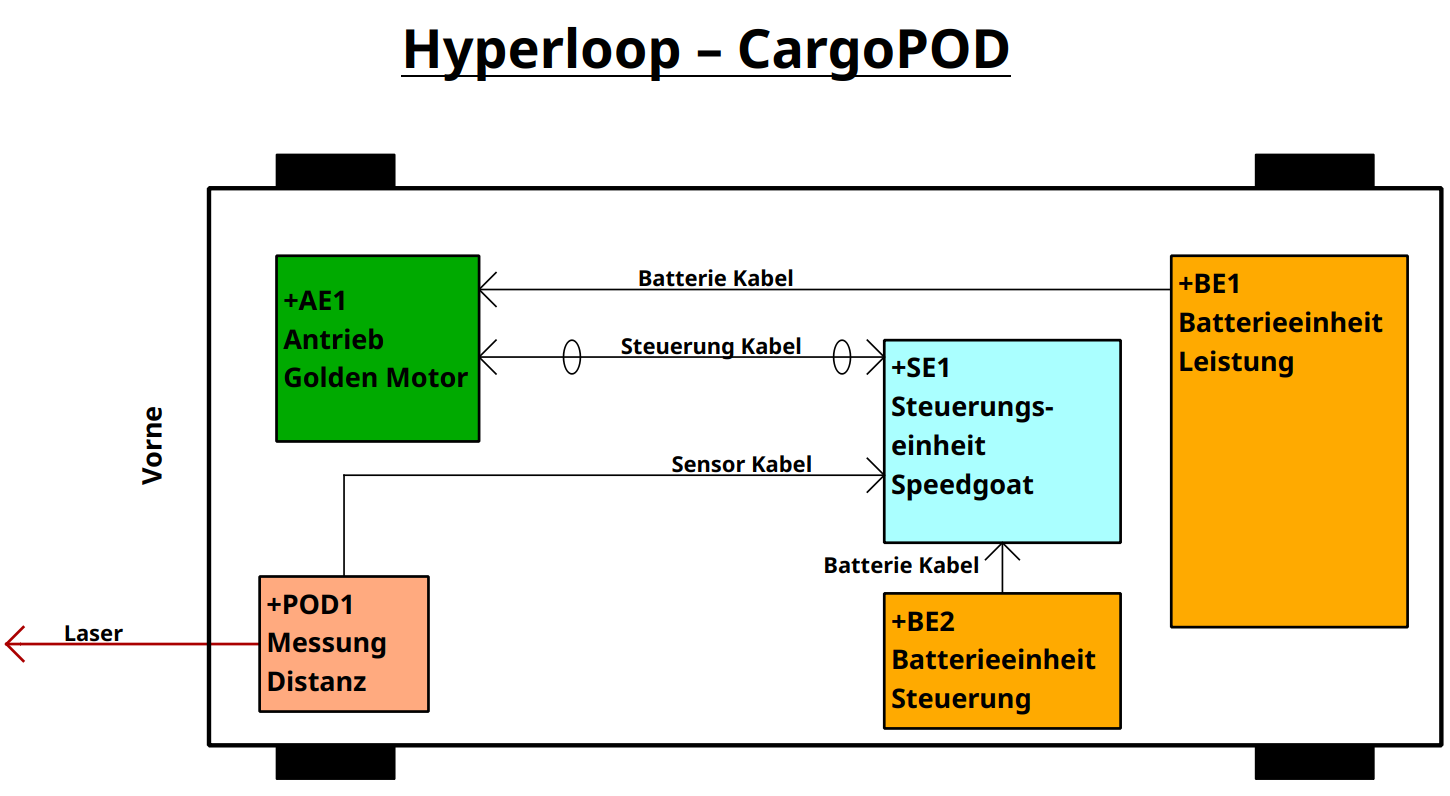
\includegraphics[width=.95\textwidth]{img/3_schaltplan/sp_aufbauplan_0.png}
		\caption{Konzept – Aufbauplan des Fahrzeugs}
		\label{img_1_1:Konzept:0}
	\end{center}
\end{figure}
\pagebreak[1]
Wie in Abbildung \ref{img_1_1:Konzept:0} dargestellt, werden die Baugruppen des Fahrzeugs an verschiedenen Stellen miteinander verbunden. Dabei übernimmt die Steuereinheit (+SE1) eine zentrale Rolle. Mit der echtzeitfähigen Steuerung von Speedgoat werden alle digitalen und analogen Ein- und Ausgangssignale gesteuert, einschließlich der Distanzmessung. Die Distanzmessung ist für die Positions- und Geschwindigkeitsermittlung notwendig. Die Steuereinheit (+SE1) wird von der Batterieeinheit (+BE2) mit Energie versorgt.\\
Der Antrieb (+AE1) erfolgt über einen BLDC-Motor. Dieser wird mittels eines zusätzlichen Steuergeräts, einem Vector-Controller, angesteuert. Für die Energieversorgung des Antriebs wird eine Leistungsbatterie (+BE1) verwendet.


\include{source/einennoch}
\chapter{Stand der Technik}
\label{chapter:Stand_der_Technik}
\myboxy{
	\begin{itemize}
		\item Bilder neu machen aus dem Schaltplan.
		\item Vector Controller, Funktionsweise nur kurz erklären und mehr auf die Anschlüsse eingehen.
		\item PIN-Mapping als Tabelle erstellen, für den Motor und den Vector Controller.
		\item QElectroTeck.
		\item PIN-Mapping als Tabelle erstellen, für den Motor und den Vector Controller.
		\item Auf die PDF verweisen.
	\end{itemize}
}{To-do}{\textwidth}



Im folgenden Abschnitt werden die verwendeten Bauteile, welche in Kapitel \ref{chapter:Konzept} dargestellt worden sind, näher beschrieben.


\section{Antrieb – Golden Motor}
\label{section:Antrieb}

Golden Motor bietet eine Gesamtlösung bestehend aus einem BLDC-Motor und einem Vektor-Controller an. Der Controller besitzt eine Schnittstelle für alle notwendigen Steuer- und Kontrollsignale, um den Motor anzutreiben. Die Anschlüsse sowie die grundlegende Funktionsweise werden in den Abschnitten \ref{section:BLDC_Motor} und \ref{section:Vector_Controller} näher erläutert.



\subsection{BLDC Motor}
\label{section:BLDC_Motor}

Der in Abbildung \ref{BLDC_Motor:img:antrieb_motor} dargestellte BLDC-Motor verfügt über eine Leistung von 10 kW und kann optional durch eine Ölkühlung gekühlt werden, was jedoch für das Fahrzeug derzeit nicht relevant ist. Die Drehzahl ist variabel und kann, mittls des Vector Controllers, welcher in Abschnitt \ref{section:Vector_Controller} erklärt wird, zwischen 2.000 und 6.000 U/min eingestellt werden. Das Nenndrehmoment beträgt 26 Nm, während das maximale Drehmoment bei 85 Nm liegt. Der Wirkungsgrad des Motors beträgt 91 \% \cite{Golden_Motor:bldc_motor}.

\pagebreak[1]
\begin{figure}[!ht]
	\begin{center}
		\includegraphics[width=1\textwidth]{img/2_antrieb/motor_1.png}
		\caption{Golden Motor – 10 KW BLDC Motor Liquid Cooled}
		\label{BLDC_Motor:img:antrieb_motor}
	\end{center}
\end{figure}


Die Anschlüsse des Motors sind in Tabelle \ref{BLDC_Motor:tab:pinmapping} aufgelistet. Der Motor verfügt über zwei Hall-Sensor-Kabel, die jeweils drei Hall-Sensoren sowie einen Temperatursensor enthalten. Zusätzlich sind ein GND- und ein +5V-Versorgungsanschluss in den Hall-Sensor-Kabeln integriert. Die Spulen des Motors werden über sechs separate Kabel angeschlossen: U, V und W.
\pagebreak[1]
\begin{table}[!ht]
	\centering
	\caption{Pin Mapping – BLDC-Motor}
	\label{BLDC_Motor:tab:pinmapping}
	\begin{tabular}{lll}
		\hline
		\textbf{Anschluss}          & \textbf{Funktionalität} & \textbf{Farbe} \\ \hline
		\multicolumn{3}{c}{\textbf{Anschluss Adern Motor}}                     \\ \hline
		\multicolumn{1}{l|}{U1}     & Spule 1                 & Gelb           \\
		\multicolumn{1}{l|}{V1}     & Spule 2                 & Grün           \\
		\multicolumn{1}{l|}{W1}     & Spule 3                 & Blau           \\
		\multicolumn{1}{l|}{U2}     & Spule 1                 & Gelb           \\
		\multicolumn{1}{l|}{V2}     & Spule 2                 & Grün           \\
		\multicolumn{1}{l|}{W2}     & Spule 3                 & Blau           \\ \hline
		\multicolumn{3}{c}{\textbf{Motor Hall Kabel 1}}                        \\ \hline
		\multicolumn{1}{l|}{Hall A} & Hall Sensor             & Gelb           \\
		\multicolumn{1}{l|}{Hall B} & Hall Sensor             & Grün           \\
		\multicolumn{1}{l|}{Hall C} & Hall Sensor             & Blau           \\
		\multicolumn{1}{l|}{Temp}   & Temperatur Sensor       & Weiß           \\
		\multicolumn{1}{l|}{+5V}    & Spannungsversorgung     & Rot            \\
		\multicolumn{1}{l|}{GND}    & Masse                   & Schwarz        \\ \hline
		\multicolumn{3}{c}{\textbf{Motor Hall Kabel 2}}                        \\ \hline
		\multicolumn{1}{l|}{Hall A} & Hall Sensor             & Gelb           \\
		\multicolumn{1}{l|}{Hall B} & Hall Sensor             & Grün           \\
		\multicolumn{1}{l|}{Hall C} & Hall Sensor             & Blau           \\
		\multicolumn{1}{l|}{Temp}   & Temperatur Sensor       & Weiß           \\
		\multicolumn{1}{l|}{+5V}    & Spannungsversorgung     & Rot            \\
		\multicolumn{1}{l|}{GND}    & Masse                   & Schwarz        \\ \hline
	\end{tabular}
\end{table}
\pagebreak[4]



\subsubsection{Funktionsweise}
\label{BLDC_Motor:Funktionsweise}
Ein BLDC-Motor (Brushless DC Motor) unterscheidet sich grundlegend von einem herkömmlichen Gleichstrommotor. Während bei einem traditionellen DC-Motor die Polumschaltung (Kommutierung) mechanisch über Kohlebürsten erfolgt, übernimmt beim BLDC-Motor eine elektronische Steuerung diese Aufgabe. Dadurch entfällt die Notwendigkeit von Kohlebürsten, was den Motor effizienter und langlebiger macht\cite{mathworks:bldc_motor}.
\newpage



\subsection{Vector Controller}
\label{section:Vector_Controller}

Der Motor wird mithilfe eines Vektor-Controllers angesteuert, der in Abbildung \ref{Vector_Controller:img:Antrieb_Controller} dargestellt ist. Der Controller hat die Aufgabe, den Motor basierend auf den Eingangssignalen so zu steuern, dass beispielsweise eine gewünschte Drehzahl erreicht wird. Die genaue Funktionsweise des Vektor-Controllers wird kurz unter \ref{Vector_Controller:Funktionsweise} erläutert.

Das Pin-Mapping ist in Tabelle \ref{Vector_Controller:tab:pinmapping} aufgeführt. Bei den Steuersignalen muss auf den Spannungsbereich geachtet werden, da der Controller eine Störung meldet, wenn ein Signal außerhalb des zulässigen Bereichs liegt. Dies ist ein integriertes Sicherheitssystem des Controllers. Dies ist ein integriertes Sicherheitssystem des Controllers. So liegt beispielsweise bei der Bremse das logische Signal bei 0, wenn die Spannung 1 V beträgt. Tritt ein Kabelbruch ein, wird die Spannung am Controller bei 0 V liegen und eine Warnung wird durch ein periodisches Tonsignal ausgegeben.


\begin{figure}[!ht]
	\begin{center}
		\includegraphics[width=1\textwidth]{img/2_antrieb/sine_1.png}
		\caption{Golden Motor – VECTOR 500 Motor Controller}
		\label{Vector_Controller:img:Antrieb_Controller}
	\end{center}
\end{figure}

\begin{table}[!ht]
	\centering
	\caption{Pin Mapping – Vector Controller}
	\label{Vector_Controller:tab:pinmapping}
	\begin{tabular}{lll|l}
		\hline
		\textbf{Anschluss}           & \textbf{Funktionalität}  & \textbf{Farbe}              & \textbf{U in V}             \\ \hline
		\multicolumn{4}{c}{\textbf{Batterie Eingang}}                                                                       \\ \hline
		\multicolumn{1}{l|}{B+}      & Versorgungsspannung      & RT                          & 48 V                        \\
		\multicolumn{1}{l|}{B-}      & Masse                    & SW                          & 0 V                         \\ \hline
		\multicolumn{4}{c}{\textbf{Motor Ausgnag}}                                                                          \\ \hline
		\multicolumn{1}{l|}{U}       & Spule 1                  & GE                          &                             \\
		\multicolumn{1}{l|}{V}       & Spule 2                  & GN                          &                             \\
		\multicolumn{1}{l|}{W}       & Spule 3                  & BL                          &                             \\ \hline
		\multicolumn{4}{c}{\textbf{Steuerungskabel}}                                                                        \\ \hline
		\multicolumn{1}{l|}{1}       & CANL - CAN-Bus           & \textcolor{red}{Vorhanden?} &                             \\
		\multicolumn{1}{l|}{2}       & CANH – CAN-Bus           & \textcolor{red}{Vorhanden?} &                             \\
		\multicolumn{1}{l|}{3}       & Motor Temperatur         & BL                          &                             \\
		\multicolumn{1}{l|}{4, 5, 6} & Masse                    & SW                          & 0 V                         \\
		\multicolumn{1}{l|}{7}       & Tempomat                 & Gr                          & 0 V - 5 V                   \\
		\multicolumn{1}{l|}{10}      & Elektronisches Schloss   & OR                          & 0 V - 5 V                   \\
		\multicolumn{1}{l|}{11}      & Hall C – Sensor          & BL                          &                             \\
		\multicolumn{1}{l|}{12}      & Hall B – Sensor          & GN                          &                             \\
		\multicolumn{1}{l|}{13}      & Hall A – Sensor          & GE                          &                             \\
		\multicolumn{1}{l|}{14}      & +5 V                     & RT                          & 5 V                         \\
		\multicolumn{1}{l|}{15}      & +12V Bremse              & GN\&WS                      & \textcolor{red}{Vorhanden?} \\
		\multicolumn{1}{l|}{16}      & Bremse                   & BL\&WS                      & 1 V - 5 V                   \\
		\multicolumn{1}{l|}{20}      & Hohe Geschwindigkeit     & BL                          & \textcolor{red}{Vorhanden?} \\
		\multicolumn{1}{l|}{21}      & Masse                    & SW                          & 0 V                         \\
		\multicolumn{1}{l|}{24}      & Niedrige Geschwindigkeit & BL                          & \textcolor{red}{Vorhanden?} \\
		\multicolumn{1}{l|}{25}      & Masse                    & SW\&WS                      & 0 V                         \\
		\multicolumn{1}{l|}{26}      & Gaspedal                 & GN\&WS                      & 1 V - 4 V                   \\
		\multicolumn{1}{l|}{27}      & Masse                    & SW                          & 0 V                         \\ \hline
	\end{tabular}
\end{table}
\pagebreak[4]

\subsubsection{Funktionsweise}
\label{Vector_Controller:Funktionsweise}
Der Vektor-Controller verwendet die Motorsteuerungstechnologie der feldorientierten Regelung (Field-Oriented Control, FOC). Dabei wird die Position des Rotors im Motor mithilfe von Hall-Sensoren ermittelt. Mit der FOC-Technik ist es möglich, das Verhältnis von Drehmoment pro Ampere zu maximieren. Dafür muss der Rotorflussvektor im rechten Winkel (90 Grad) zum Statorflussvektor ausgerichtet sein \cite{Golden_Motor:Vector_Controller}.


\newpage


\section{Echtzeitfähige Steuerung – Speedgoat}
\label{section:speedgoat}
\myboxy{
	\begin{itemize}
		\item I/O Module 691 zuende Erklären.
		\item Echtzeitfähigkeit auf die DIN Norm beziehen und besser erklären auf unserer Situation.
	\end{itemize}
}{To-do}{\textwidth}

Der Baseline Real-Time Target Machine, wie in Abbildung \ref{speedgoat:img:steuerung_goat} dargestellt, ist ein echtzeitfähiges System, welches ovn der Firma Speedgoat hergestellt und vertrieben wirden. Es wird hauptsächlich in der Entwicklung und beim Testen von komplexen Steuerungs- und Regelungssystemen eingesetzt, bei denen die Echtzeitfähigkeit eine zentrale Rolle spielt.\\ \ \\


\pagebreak[1]
\begin{figure}[!ht]
	\begin{center}
		\includegraphics[width=1\textwidth]{img/2_steuerung/goat_1.png}
		\caption{Speedgoat – Baseline Real-Time Target Machine}
		\label{speedgoat:img:steuerung_goat}
	\end{center}
\end{figure}
\pagebreak[1]

Speedgoat-Systeme integrieren sich nahtlos mit Simulink, einer Software von MathWorks, die häufig zur Modellierung und Simulation dynamischer Systeme verwendet wird. Durch eine große Auswahl an I/O-Modulen lassen sich verschiedene Sensoren und Aktuatoren problemlos an die Systeme anschließen.
Echtzeitsysteme von Speedgoat sind Computer, die in der Lage sind, Aufgaben innerhalb festgelegter Zeitintervalle auszuführen. Diese Systeme sind entscheidend für Anwendungen, bei denen die zeitliche Genauigkeit von großer Bedeutung ist, wie beispielsweise bei der Steuerung von Motoren, der Regelung von Prozessen oder der Simulation von physikalischen Systemen.


\pagebreak[1]
\begin{figure}[!ht]
	\begin{center}
		\includegraphics[width=1\textwidth]{img/2_steuerung/goat_2.png}
		\caption{Speedgoat – Ansicht der Modulanschlüsse}
		\label{speedgoat:img:Modulanschlüsse}
	\end{center}
\end{figure}
\pagebreak[1]
In Abbildung \ref{speedgoat:img:Modulanschlüsse} sind die Anschlüsse der I/O-Module des Speedgoat-Systems dargestellt. Die Zuordnung der Module zu den entsprechenden Anschlüssen ist in Tabelle \ref{speedgoat:tab:Module} ersichtlich.

Das Modul IO397-50k-50k kann über ein Sensor-Aktor-Kabel von Phoenix Contact extern angeschlossen werden, wie in Abbildung \ref{IO397_50k:img:Module} dargestellt.
Zusätzlich wird das Modul IO691 mittels eines 9-Pin D-Sub-Steckers angeschlossen.
\pagebreak[1]
\begin{table}[!ht]
	\centering
	\caption{Speedgoat – Anschlüsse der Module}
	\label{speedgoat:tab:Module}
	\begin{tabular}{clll}
		\hline
		\multicolumn{2}{c}{\textbf{I/O Module}} & \multicolumn{1}{c}{\textbf{Name}} & \textbf{Funktion}               \\ \hline
		\multirow{2}{*}{1}                      & \multicolumn{1}{l|}{A}            & IO397-50k         & analog I/O  \\
		                                        & \multicolumn{1}{l|}{B}            & IO397-50k         & digital I/O \\ \hline
		\multirow{2}{*}{2}                      & \multicolumn{1}{l|}{A}            & IO691             & CAN         \\
		                                        & \multicolumn{1}{l|}{B}            & IO691             & CAN         \\ \hline
		\multirow{2}{*}{3}                      & \multicolumn{1}{l|}{A}            & IO397-50k         & analog I/O  \\
		                                        & \multicolumn{1}{l|}{B}            & IO397-50k         & digital I/O \\ \hline
		\multirow{2}{*}{4}                      & \multicolumn{1}{l|}{A}            & Frei              &             \\
		                                        & \multicolumn{1}{l|}{B}            & Frei              &             \\ \hline
	\end{tabular}
\end{table}
\pagebreak[4]




\subsection{I/O-Modul – IO397-50k}
\label{section:IO397_50k}

Das in Abbildung \ref{IO397_50k:img:Module} dargestellte IO397-50k I/O-Modul verfügt über zahlreiche analoge und digitale Ein- sowie Ausgänge. Die Anschlüsse werden auf Modul A, das die analogen Schnittstellen bereitstellt, und Modul B, welches die digitalen Schnittstellen umfasst, verteilt. Die Anschlussbelegung werden in den Tabellen \ref{IO397_50k:tab:Board_A} und \ref{IO397_50k:tab:Board_B} dargestellt. Die Spannungen der Ein- und Ausgänge können softwaregesteuert angepasst werden \cite{speedgoat:IO397_50k}.

\pagebreak[1]
\begin{figure}[!ht]
	\begin{center}
		\includegraphics[width=0.7\textwidth]{img/2_steuerung/goat_io397.png}
		\caption{Speedgoat – I/O Module 397 \cite{speedgoat:IO397_50k}}
		\label{IO397_50k:img:Module}
	\end{center}
\end{figure}
\pagebreak[1]

\subsubsection{Pin Mapping – IO397-50k}


Das Terminal Board A ist für die Verarbeitung analoger Signale konzipiert, sowohl für Eingänge als auch für Ausgänge. Die Tabelle \ref{IO397_50k:tab:Board_A} zeigt das Pin-Mapping von Terminal Board A. Dieses Board verfügt über Anschlüsse für insgesamt vier analoge Eingänge (Pins A1 bis A8) und vier analoge Ausgänge (Pins A9 bis A12). Die Ausgänge sind an einen Digital-zu-Analog-Wandler (DAC) angeschlossen, während die Eingänge mit einem Analog-zu-Digital-Wandler (ADC) verbunden sind.

\pagebreak[1]
\begin{table}[!ht]
	\centering
	\caption{IO397-50k Pin Mapping – Terminal Board A: analog I/O \cite[15]{speedgoat:IO397_50k}}
	\label{IO397_50k:tab:Board_A}
	\begin{tabular}{lll}
		\hline
		\textbf{Pin}             & \textbf{Funktionalität} & \textbf{Type} \\ \hline
		\multicolumn{1}{l|}{A1}  & Analog input 1 +        & ADC           \\
		\multicolumn{1}{l|}{A2}  & Analog input 1 -        & ADC           \\
		\multicolumn{1}{l|}{A3}  & Analog input 2 +        & ADC           \\
		\multicolumn{1}{l|}{A4}  & Analog input 2 -        & ADC           \\
		\multicolumn{1}{l|}{A5}  & Analog input 3 +        & ADC           \\
		\multicolumn{1}{l|}{A6}  & Analog input 3 -        & ADC           \\
		\multicolumn{1}{l|}{A7}  & Analog input 4 +        & ADC           \\
		\multicolumn{1}{l|}{A8}  & Analog input 4 -        & ADC           \\ \hline
		\multicolumn{1}{l|}{A9}  & Analog output 1         & DAC           \\
		\multicolumn{1}{l|}{A10} & Analog output 2         & DAC           \\
		\multicolumn{1}{l|}{A11} & Analog output 3         & DAC           \\
		\multicolumn{1}{l|}{A12} & Analog output 4         & DAC           \\ \hline
		\multicolumn{1}{l|}{A13} & GND                     & GND           \\
		\multicolumn{1}{l|}{A14} & GND                     & GND           \\
		\multicolumn{1}{l|}{A15} & 0 V                     & 0 V           \\
		\multicolumn{1}{l|}{A16} & 5 V DC                  & 5 V DC        \\
		\multicolumn{1}{l|}{A17} & GND                     & GND           \\
		\multicolumn{1}{l|}{SH}  & SH                      & Shielding     \\ \hline
	\end{tabular}
\end{table}
\pagebreak[1]


Terminal Board B hingegen bietet eine flexible Konfiguration für digitale Ein- und Ausgänge. Die Tabelle \ref{IO397_50k:tab:Board_B} zeigt das Pin Mapping von Terminal Board B. Die Pins B3 bis B16 sind für konfigurierbare I/O-Funktionalitäten ausgelegt und nutzen TTL-Signale (Transistor-Transistor-Logik), was sie besonders für schnelle digitale Schaltvorgänge geeignet macht. Dieses Board ermöglicht es, die Anschlüsse flexibel zu nutzen, je nach den Anforderungen der Applikation. Auch hier gibt es mehrere Spannungs- und Ground-Anschlüsse, sowie eine Abschirmung (Shielding) für das M12-Kabel, um elektromagnetische Störungen zu minimieren.


\pagebreak[1]
\begin{table}[!ht]
	\centering
	\caption{IO397-50k Pin Mapping – Terminal Board B: analog I/O \cite[15]{speedgoat:IO397_50k}}
	\label{IO397_50k:tab:Board_B}
	\begin{tabular}{lll}
		\hline
		\textbf{Pin}             & \textbf{Funktionalität} & \textbf{Type} \\ \hline
		\multicolumn{1}{l|}{B1}  & 0 V                     & 0 V           \\
		\multicolumn{1}{l|}{B2}  & 5 V DC                  & 5 V DC        \\ \hline
		\multicolumn{1}{l|}{B3}  & I/O 0                   & IN/OUT        \\
		\multicolumn{1}{l|}{B4}  & I/O 1                   & IN/OUT        \\
		\multicolumn{1}{l|}{B5}  & I/O 2                   & IN/OUT        \\
		\multicolumn{1}{l|}{B6}  & I/O 3                   & IN/OUT        \\
		\multicolumn{1}{l|}{B7}  & I/O 4                   & IN/OUT        \\
		\multicolumn{1}{l|}{B8}  & I/O 5                   & IN/OUT        \\
		\multicolumn{1}{l|}{B9}  & I/O 6                   & IN/OUT        \\
		\multicolumn{1}{l|}{B10} & I/O 7                   & IN/OUT        \\
		\multicolumn{1}{l|}{B11} & I/O 8                   & IN/OUT        \\
		\multicolumn{1}{l|}{B12} & I/O 9                   & IN/OUT        \\
		\multicolumn{1}{l|}{B13} & I/O 10                  & IN/OUT        \\
		\multicolumn{1}{l|}{B14} & I/O 11                  & IN/OUT        \\
		\multicolumn{1}{l|}{B15} & I/O 12                  & IN/OUT        \\
		\multicolumn{1}{l|}{B16} & I/O 13                  & IN/OUT        \\\hline
		\multicolumn{1}{l|}{B17} & GND                     & GND           \\
		\multicolumn{1}{l|}{B18} & SH                      & Shielding     \\ \hline
	\end{tabular}
\end{table}
\pagebreak[4]


\subsubsection{IO397-50k – Konfigurieren}
\label{Simulink:IO397_50k_Konfigurieren}

In dem Driver Block, wie in Abbildung \ref{IO397_50k_Konfigurieren:img:Driver_Block} gezeigt, können am dem Pull-Widerstand des I/O-Moduls verschiedene Spannungen eingestellt werden. Zur Auswahl stehen:
\begin{itemize}
	\item Pull-up 3,3 V
	\item Weak Pull-up 5,0 V
	\item Pull-down
	\item Floating
\end{itemize}
welche im Folgenden erklärt werden.

\pagebreak[1]
\begin{figure}[!ht]
	\begin{center}
		\includegraphics[width=.5\textwidth]{img/4_simulink/IO397_50k.png}
		\caption{Simulink – Driver Block – IO397-50k}
		\label{IO397_50k_Konfigurieren:img:Driver_Block}
	\end{center}
\end{figure}
\pagebreak[1]

Pull-Widerstände werden verwendet, um klare digitale Schaltzustände zu gewährleisten. Es gibt drei verschiedene Zustände: \frqq High\flqq\ entspricht \frqq logisch 1\flqq\, Low entspricht \frqq logisch 0\flqq\. \frqq Floating\flqq\ hat die Bedeutung, dass der Widerstand nicht an \frqq GND\flqq\ oder an einer Spannung angeschlossen ist. Somit ist der Widerstand hochohmig. Die Zustände zu den Einstellungen sind in der Tabelle \ref{IO397_50k_Konfigurieren:tab:Reaktionszeit} aufgeführt.
In Abbildung \ref{IO397_50k_Konfigurieren:img:TTL_IO_Interface} ist im rot markierten Bereich der Pull-Widerstand mit 4,7 k$\Omega$ an einen 47-$\Omega$-Widerstand am I/O-Anschluss angeschlossen. Der Pull-Widerstand kann, wie bereits erwähnt, konfiguriert werden. Dabei wird intern am Pull-Widerstand entweder eine Spannung von 3,3 V, 5 V, GND oder kein Kontakt, also Floating (hochohmig), geschaltet.

\pagebreak[1]
\begin{figure}[!ht]
	\begin{center}
		\includegraphics[width=1.1\textwidth]{img/4_simulink/TTL_IO_Interface.png}
		\caption{Speedgoat – TTL I/O Interface – IO397-50k \cite[12]{speedgoat:IO397_50k}}
		\label{IO397_50k_Konfigurieren:img:TTL_IO_Interface}
	\end{center}
\end{figure}
\pagebreak[2]



Bei der Einstellung auf 3,3 V oder 5 V fungiert der Widerstand als Pull-up-Widerstand. Bei der Pull-down-Konfiguration liegt am Widerstand Ground (GND) an.



In Tabelle \ref{IO397_50k_Konfigurieren:tab:Reaktionszeit} können die Reaktionszeiten der digitalen Ausgänge verglichen werden. Bei der Einstellung \frqq Weak Pull-up 5,0 V\flqq\ bedeutet \frqq weak\flqq, dass der Ausgang eine langsamere Anstiegszeit hat. In Abbildung \ref{IO397_50k_Konfigurieren:img:Pull_Widerstande} sind die Reaktionszeiten dargestellt.


\pagebreak[1]
\begin{table}[!ht]
	\centering
	\caption{Simulink – Pull-Widerstand – Reaktionszeit}
	\label{IO397_50k_Konfigurieren:tab:Reaktionszeit}
	\begin{tabular}{lccc}
		\hline
		\multicolumn{1}{c}{\multirow{2}{*}{\textbf{Einstellung}}} & \multicolumn{1}{c}{\multirow{2}{*}{\textbf{Logischer zustand}}} & \multicolumn{2}{c}{\textbf{Reaktionszeit der Ausgänge}}           \\ \cline{3-4}
		\multicolumn{1}{c}{}                                      & \multicolumn{1}{c}{}                                            & Anstieg                                                 & Abfall  \\ \hline
		\multicolumn{1}{l|}{Pull-up 3,3V}                         & I/O = 1                                                         & Schnell                                                 & Schnell \\
		\multicolumn{1}{l|}{weak pull-up 5,0V}                    & I/O = 1                                                         & Langsam                                                 & Schnell \\
		\multicolumn{1}{l|}{Pull-down}                            & I/O = 0                                                         & Schnell                                                 & Langsam \\
		\multicolumn{1}{l|}{Floating}                             & I/O = 0 - 1                                                     & -                                                       & -       \\ \hline
	\end{tabular}
\end{table}
\pagebreak[1]



\pagebreak[1]
\begin{figure}
	\begin{minipage}{0.8\textwidth}
		\centering
		\includegraphics[width=1\textwidth]{img/4_simulink/O_Interface_3V3.png}
		\caption*{Pull-up-Widerstand 3,3 V}
	\end{minipage}
	\begin{minipage}{0.8\textwidth}
		\centering
		\includegraphics[width=1\textwidth]{img/4_simulink/O_Interface_5V.png}
		\caption*{Weak Pull-up-Widerstand 5 V}
	\end{minipage}
	\begin{minipage}{0.8\textwidth}
		\centering
		\includegraphics[width=1\textwidth]{img/4_simulink/O_Interface_0V.png}
		\caption*{Pull-down-Widerstand GND}
	\end{minipage}
	\caption{Simulink – Pull-Widerstände – IO397-50k \cite[12]{speedgoat:IO397_50k}}
	\label{IO397_50k_Konfigurieren:img:Pull_Widerstande}
\end{figure}
\pagebreak[4]

\newpage
\subsection{I/O-Modul – IO691}
\label{section:IO691}

Das IO691 I/O-Modul bietet eine intelligente CAN-Schnittstelle mit zwei Kanälen, die sowohl flexible Datenrate CAN (CAN FD) als auch High-Speed CAN (CAN HS) unterstützen. Es ist kompatibel mit CAN 2.0A/B-Netzwerken und unterstützt SAE J1939 sowie ASAM XCP für Bypassing. Alle Signale sind über 9-polige D-Sub-Front-CAN-Anschlüsse zugänglich \cite[4]{speedgoat:IO691}.

\pagebreak[1]
\begin{figure}[!ht]
	\begin{center}
		\includegraphics[width=0.7\textwidth]{img/2_steuerung/goat_io691.png}
		\caption{Speedgoat – I/O Module 691 \cite{speedgoat:IO691}}
		\label{img_2_2:goat:IO691}
	\end{center}
\end{figure}
\pagebreak[4]




\subsubsection{Pin Mapping –  IO691}

\pagebreak[1]
\begin{table}[!ht]
	\centering
	\caption{IO691 Pin Mapping}
	\label{speedgoat:IO691}
	\begin{tabular}{lllc}
		\hline
		\textbf{Pin}            & \textbf{Farbe} & \textbf{An Sensor} & \textbf{DB9 Connector A/B, Signal} \\ \hline
		\multicolumn{1}{l|}{1}  & Braun          & PIN 2 -  Weiß      & Vcc                                \\
		\multicolumn{1}{l|}{2}  & Rot            & PIN 5 -  Grau      & CAN-low                            \\
		\multicolumn{1}{l|}{3}  & Orange         & PIN 3 -  Blau      & GND                                \\
		\multicolumn{1}{l|}{4}  & Gelb           &                    & -                                  \\
		\multicolumn{1}{l|}{5}  & Grün           &                    & -                                  \\
		\multicolumn{1}{l|}{6}  & Blau           & PIN 3 -  Blau      & GND                                \\
		\multicolumn{1}{l|}{7}  & Viollet        & PIN 4 -  Schwarz   & CAN-high                           \\
		\multicolumn{1}{l|}{8}  & Grau           &                    & -                                  \\
		\multicolumn{1}{l|}{9}  & Schwarz        &                    & -                                  \\
		\multicolumn{1}{l|}{SH} &                & PIN 1 - Braun      & Shield                             \\ \hline
	\end{tabular}
\end{table}
\pagebreak[1]


\subsubsection{IO691 Module Konfigurieren}
\label{Simulink:IO691_Konfigurieren}

Im \frqq Driver Block\flqq, siehe Abbildung \ref{IO691_Konfigurieren:img:Driver_Block}, können die \frqq CAN Channels\flqq\ 1 und 2 konfiguriert werden. Wie bereits in Abschnitt \ref{section:IO691} erwähnt, lässt sich der Protokollmodus jedes Kanals separat einstellen, wobei zwischen \frqq CAN HS\flqq, \frqq CAN FD\flqq\ und \frqq Disable\flqq\ gewählt werden kann. Dabei entspricht \frqq CAN HS\flqq\ der Norm ISO 11898-2 und \frqq CAN FD\flqq\ der Norm ISO 11898-1 \cite[4]{speedgoat:IO691}.

\pagebreak[1]
\begin{figure}[!ht]
	\begin{center}
		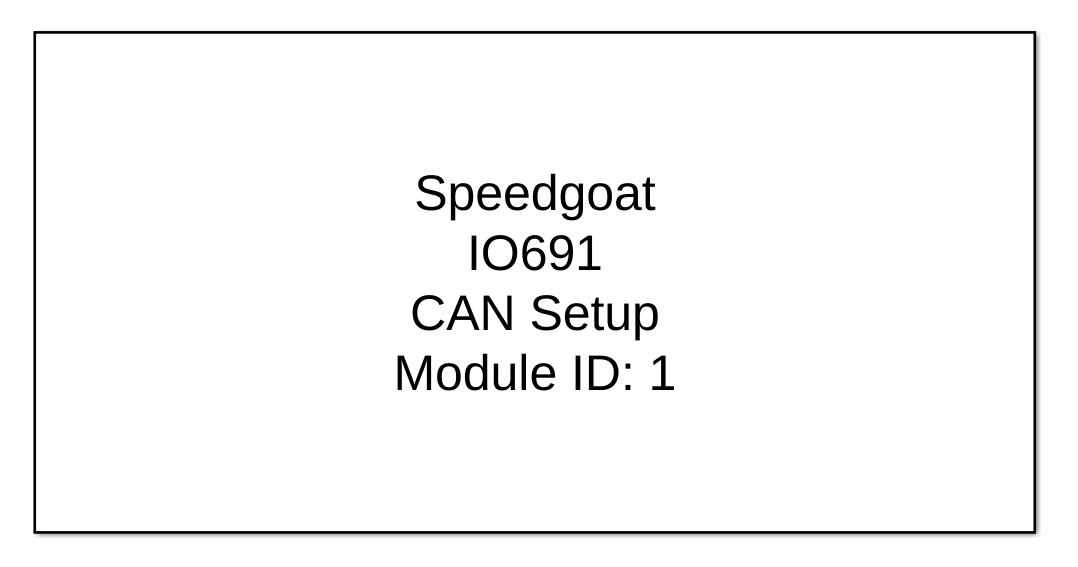
\includegraphics[width=0.7\textwidth]{img/4_simulink/IO691.png}
		\caption{Simulink – Driver Block – I/O Module 691 \cite{speedgoat:IO691}}
		\label{IO691_Konfigurieren:img:Driver_Block}
	\end{center}
\end{figure}
\pagebreak[1]


Die \frqq Initialization\flqq- und \frqq Termination\flqq-CAN-Nachrichten können individuell angepasst werden. Im nachfolgenden Matlab-Skript (\ref{IO691_Konfigurieren:code:Driver_Block}) werden die Variablen \frqq initCAN\flqq\ und \frqq termCAN\flqq\ definiert.



\pagebreak[4]
\begin{lstlisting}[language=Matlab, caption=Initialization and Termination Structure \cite{speedgoat:IO691:CAN_Message}\label{IO691_Konfigurieren:code:Driver_Block}]
% create Initialization structure
initCAN.Channel     = 1;
initCAN.Protocol    = 'CAN-FD';         % 'CAN' or 'CAN-FD'
initCAN.BRS         = 1;                % 0 or 1
initCAN.Type        = 'Standard';       % 'Standard' or 'Extended'
initCAN.Identifier  = 99;               % ID must be double
initCAN.Data        = [8 8 8 8 8 8 8 8];
initCAN.Pause       = 0.05;

% create Termination structure
termCAN.Channel     = 1;
termCAN.Protocol    = 'CAN-FD';         % 'CAN' or 'CAN-FD'
termCAN.BRS         = 1;                % 0 or 1
termCAN.Type        = 'Extended';       % 'Standard' or 'Extended'     
termCAN.Identifier  = double(0xFFF);    % ID must be double
termCAN.Data        = [1 1 1 1 1 1 1 1];
termCAN.Pause       = 0.05



 
\end{lstlisting}
\pagebreak[1]

Die Baudrate kann in zwei Kategorien unterteilt werden: \frqq Nominal Baud Rate\flqq\ und \frqq Data Baud Rate\flqq. Wenn im \frqq CAN Channels\flqq-Menü der Modus \frqq CAN FD\flqq\ ausgewählt wird, können beide Baudraten konfiguriert werden. Im Modus \frqq CAN HS\flqq\ ist die Einstellung der \frqq Nominal Baud Rate\flqq\ möglich. \\
Es können entweder die voreingestellten Baudraten verwendet oder eigene Werte über ein Array [BRP, SJW, TSEG1, TSEG2] konfiguriert werden, deren Elemente im Folgenden kurz erläutert werden, siehe Tabelle \ref{IO691_Konfigurieren:tab:Baudraten}.

\pagebreak[1]
\begin{table}[!ht]
	\centering
	\caption{Simulink – Baudraten Parameter }
	\label{IO691_Konfigurieren:tab:Baudraten}
	\begin{tabular}{ll}
		\hline
		\multicolumn{1}{c}{\textbf{Abkürzung}} & \multicolumn{1}{c}{\textbf{Bedeutung}} \\ \hline
		\multicolumn{1}{l|}{BRP}               & Bit Rate Prescaler                     \\
		\multicolumn{1}{l|}{SJW}               & Synchronization Jump Width             \\
		\multicolumn{1}{l|}{TSEG1}             & Time Segment 1                         \\
		\multicolumn{1}{l|}{TSEG2}             & Time Segment 2                         \\ \hline
	\end{tabular}
\end{table}
\pagebreak[1]



Die sogenannte \frqq CAN Nominal Bit Time\flqq, wie in Abbildung \ref{IO691_Konfigurieren:img:Baudrate} dargestellt, besteht aus vier Segmenten: dem \frqq Sync Segment\flqq, dem \frqq Propagation Segment\flqq, dem \frqq\ Phase Buffer Segment 1\flqq\ und dem \frqq Phase Buffer Segment 2\flqq.
Das \frqq Sync Segment\flqq\ dient zur Synchronisation der Knoten auf dem Bus und hat eine Länge von genau einem Zeitquantum.
Im \frqq Propagation Segment\flqq\ werden die physikalischen Verzögerungen im Busnetzwerk ausgeglichen \cite[1]{microchip:CANModule}.\\
Im \frqq Phase Buffer Segment 1\flqq\ werden positive Phasenfehler kompensiert, und das Segment kann während der Resynchronisation verlängert werden. Im \frqq Phase Buffer Segment 2\flqq\ hingegen werden negative Phasenfehler kompensiert, und das Segment kann während der Resynchronisation verkürzt werden.\\ \ \\



Der \frqq BRP\flqq\ ist ein Parameter, der das Zeitquant $t_q$ festlegt siehe Gleichung \ref{eq:tq}.
Der \frqq SJW\flqq\ ist ein Parameter, der die Länge von \frqq TSEG1\flqq\ verlängern und die Länge von \frqq TSEG2\flqq\ verkürzen kann, um die Synchronisation zwischen den Knoten zu gewährleisten, dabei darf \frqq SJW\flqq\ kleiner gleich \frqq TSEG2\flqq\ sein \cite{speedgoat:IO691:CAN_Message}.

Der Sample Point (SP) ist der Punkt innerhalb eines CAN-Bits, an dem die tatsächliche Datenabtastung stattfindet. Dieser Punkt kann durch das Verhältnis zwischen \frqq TSEG1\flqq\ und \frqq TSEG2\flqq\ angepasst werden.

\pagebreak[1]
\begin{figure}[!ht]
	\begin{center}
		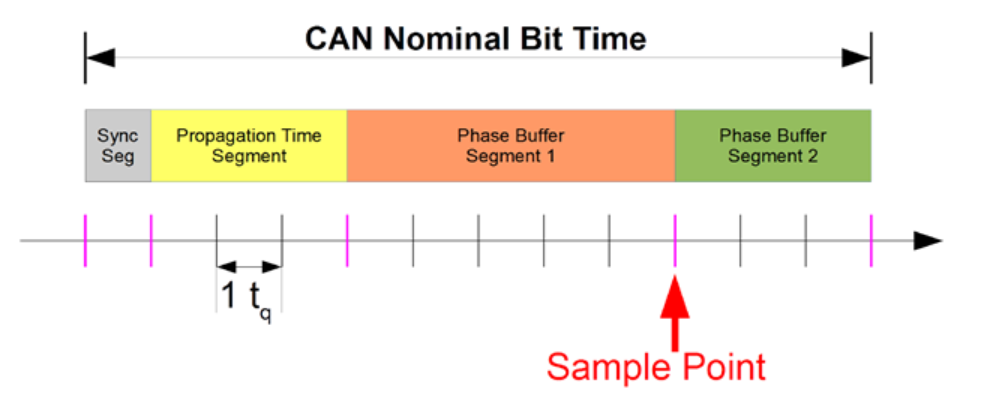
\includegraphics[width=1\textwidth]{img/4_simulink/IO691_Baudrate.png}
		\caption{Simulink – Baudrate – I/O Module 691 \cite{speedgoat:IO691:CAN_Message}}
		\label{IO691_Konfigurieren:img:Baudrate}
	\end{center}
\end{figure}
\pagebreak[1]

Mit den weiteren Gleichungen können die Zeiten innerhalb des \frqq CAN Nominal Bit Time\flqq\ ermittelt werden.
\begin{align}
	\label{eq:tq}
	t_{q}   & = \frac{BRP}{CAN_{Clk}} \\
	t_{BS1} & = t_{q}  \cdot TSEG1    \\
	t_{BS2} & = t_{q}  \cdot TSEG2
\end{align}

\begin{align}
	\begin{split}
		NominalBitTime & = t_{q} + t_{BS1} + t_{BS2}        \\
		               & = t_{q}  \cdot (1 + TSEG1 + TSEG2)
	\end{split}
\end{align}

\begin{align}
	CAN_{Baudrate} & = \frac{1}{NominalBitTime}
\end{align}

\begin{align}
	\begin{split}
		SP & = \frac{(1 + TSEG1)}{(1 + TSEG1 + TSEG2)} \\
		   & = \frac{(t_q + t_{BS1})}{NominalBitTime}
	\end{split}
\end{align}

Am CAN-Bus ist es wichtig, an beiden Enden Abschlusswiderstände von 120 $\Omega$ zu installieren. Diese Widerstände verhindern Reflexionen von Signalen, die auf der Leitung entstehen können, wenn die Impedanz des Busses nicht korrekt abgestimmt ist.\\
Reflexionen können das ursprüngliche Signal beeinträchtigen und zu Fehlern in der Datenkommunikation führen. Die Abschlusswiderstände gewährleisten eine angepasste Impedanz und minimieren somit die Wahrscheinlichkeit von Signalreflexionen \cite{speedgoat:IO691:CAN_Message}.

\include{source/einennoch}
\chapter{Implementierung}
\label{chapter:Implementierung}

\section{Schaltplan}
\label{section:Schaltplan}
Zu Beginn der Erstellung des Schaltplans sollten die Funktions- und Ortskennzeichen sowie die Beschriftung der Bauteile und Leitungen festgelegt werden. Bei der Verdrahtung ist es erforderlich, die Aderfarben den entsprechenden Spannungspotenzialen zuzuordnen.

\subsection{Betriebsmittelbezeichnung}
\label{Schaltplan:BMK}

Ein Betriebsmittel besteht aus verschiedenen Kennzeichen: dem Funktionskennzeichen (=), dem Ortskennzeichen (+) und dem Betriebsmittelkennzeichen (-). Früher wurde das Funktionskennzeichen als „Anlage“ bezeichnet. In der neuen DIN EN IEC 81346-2 \cite{DIN_EN_IEC_81346-2} wurde diese Bezeichnung jedoch auf „Funktion“ geändert.

\subsubsection{Funktionskennzeichen}
Das Funktionskennzeichen beschreibt eine bestimmte Funktion im Schaltplan, wie beispielsweise die Spannungsversorgung oder die Steuerung (siehe Tabelle \ref{BMK:tab:funktionskennzeichen}).

\pagebreak[1]
\begin{table}[!ht]
	\centering
	\caption{Schaltplan – Funktionskennzeichen (=)}
	\label{BMK:tab:funktionskennzeichen}
	\begin{tabular}{ll}
		\hline
		\textbf{Abkürzung}      & \textbf{Bezeichnung} \\ \hline
		\multicolumn{1}{l|}{SV} & Spannungsversorung   \\
		\multicolumn{1}{l|}{ST} & Steuerung            \\
		\multicolumn{1}{l|}{ES} & Eingänge Steuerung   \\
		\multicolumn{1}{l|}{AS} & Ausgänge Steuerung   \\
		\multicolumn{1}{l|}{KL} & Klemmenleisten       \\
		\multicolumn{1}{l|}{KO} & Kommunikation        \\
		\multicolumn{1}{l|}{AT} & Antrieb              \\
		\multicolumn{1}{l|}{NA} & Not-Aus              \\ \hline
	\end{tabular}
\end{table}
\pagebreak[1]

\subsubsection{Ortskennzeichen}
Das Ortskennzeichen gibt an, an welchem Ort ein Bauteil installiert ist. Beispielsweise gibt es im Fahrzeug eine Steuereinheit und eine Batterieeinheit. Im Schaltplan wird dadurch deutlich, welche Verbindungen zwischen verschiedenen Orten bestehen. Das Ortskennzeichen erleichtert zudem die Wartung und Installation des Systems.

\pagebreak[1]
\begin{table}[!ht]
	\centering
	\caption{Schaltplan – Ortskennzeichen (+)}
	\label{bmk:tab:ortskennzeichen}
	\begin{tabular}{ll}
		\hline
		\textbf{Abkürzung}       & \textbf{Bezeichnung} \\ \hline
		\multicolumn{1}{l|}{POD} & Fahrzeug             \\
		\multicolumn{1}{l|}{BE}  & Batterieeinheit      \\
		\multicolumn{1}{l|}{SE}  & Steuereinheit        \\
		\multicolumn{1}{l|}{AE}  & Antriebseinheit      \\ \hline
	\end{tabular}
\end{table}
\pagebreak[1]

\subsubsection{Betriebsmittelkennzeichen}
Das Betriebsmittelkennzeichen bezeichnet das spezifische Bauteil. Die genaue Zuordnung der Bezeichnungen ist in der DIN EN IEC 81346-2 geregelt. Die für das Projekt relevanten Betriebsmittelkennzeichen sind in Tabelle \ref{bmk:tab:betriebsmittelkennzeichen} aufgeführt.



\pagebreak[1]
\begin{table}[!ht]
	\centering
	\caption{Schaltplan – Betriebsmittelkennzeichen (-) \cite{DIN_EN_IEC_81346-2}}
	\label{bmk:tab:betriebsmittelkennzeichen}
	\begin{tabular}{|l|lll|}
		\hline
		\textbf{Abkürzung}       & \textbf{Klassenname}                            & \multicolumn{1}{l|}{\makecell[l]{\textbf{Allgemeine} \\ \textbf{Bedeutung}}} \\ \hline
		\multicolumn{1}{|l|}{FC} & \makecell[l]{Überstromschutzobjekt}             & \multicolumn{1}{l|}{Sicherung}                       \\ \hline
		\multicolumn{1}{|l|}{GB} & \makecell[l]{Erzeugungsobjekt für elektrische                                                          \\Energie durch chemische Energie} & \multicolumn{1}{l|}{Batterie} \\ \hline
		\multicolumn{1}{|l|}{KE} & \makecell[l]{Elektrische Signale                                                                       \\verarbeitendes Objekt}   & \multicolumn{1}{l|}{Steuerung} \\ \hline
		\multicolumn{1}{|l|}{MA} & \makecell[l]{Elektromagnetisches                                                                       \\Rotationsantriebsobjekt} & \multicolumn{1}{l|}{Motor} \\ \hline
		\multicolumn{1}{|l|}{QA} & \makecell[l]{Stromsteuerungsobjekt}             & \multicolumn{1}{l|}{Relais}                          \\ \hline
		\multicolumn{1}{|l|}{RL} & \makecell[l]{Bewegungsbegrenzungsobjekt}        & \multicolumn{1}{l|}{Bremse}                          \\ \hline
		\multicolumn{1}{|l|}{SF} & \makecell[l]{Fingerinteraktionsobjekt}          & \multicolumn{1}{l|}{Schalter}                        \\ \hline
		\multicolumn{1}{|l|}{TB} & \makecell[l]{Stromkonvertierungsobjekt}         & \multicolumn{1}{l|}{Transformator}                   \\ \hline
		\multicolumn{1}{|l|}{WD} & \makecell[l]{Niederspannungsenergie Leitobjekt} & \multicolumn{1}{l|}{Leitung/Kabel}                   \\ \hline
		\multicolumn{1}{|l|}{XD} & \makecell[l]{Niederspannungs-Verbindungsobjekt} & \multicolumn{1}{l|}{\makecell[l]{Klemme, Stecker     \\ oder Buchse}} \\ \hline
	\end{tabular}
\end{table}
\pagebreak[1]

Bei einer vollständigen Betriebsmittelbezeichnung sieht das Kennzeichen des Betriebsmittels folgendermaßen aus:

\begin{center} =ES2+SE1-10QA1 \end{center}

Die Betriebsmittelbezeichnung =ES2+SE1-10QA4 besagt, dass es sich um die Eingänge der Steuerung (=ES) handelt und es gibt zwei Funktionen in dem Schaltplan. Der Ort ist in der Steuereinheit (+SE) verortet, und das Betriebsmittel selbst ist ein Relais, welche auf der Seite 10 des Schaltplans zu finden ist.

Das Kennzeichen umfasst sowohl das Funktions- als auch das Ortskennzeichen, die jeweils mit einer fortlaufenden Nummer versehen werden. Das Betriebsmittelkennzeichen enthält zwei Nummerierungen: Die erste gibt an, auf welcher Seite des Schaltplans sich das Betriebsmittel befindet, während die zweite die fortlaufende Nummerierung des Bauteils darstellt.\\
Im Schaltplan wird das Betriebsmittel lediglich durch das Betriebsmittelkennzeichen (-) dargestellt, während das Funktions- und Ortskennzeichen im Zeichnungskopf angegeben ist.

\newpage

\subsection{Verdrahtung Konventionen}
\label{section:Verdrahtung_Konventionen}
Für die Verdrahtung müssen den Spannungspotenzialen verschiedene Farben zugewiesen werden. Diese Zuordnungen sind in Tabelle \ref{Verdrahtung_Konventionen:tab:Zuordnung} aufgeführt.
\pagebreak[1]
\begin{table}[!ht]
	\centering
	\caption{Verdrahtung Konvention – Aderfarben}
	\label{Verdrahtung_Konventionen:tab:Zuordnung}
	\begin{tabular}{lccl}
		\hline
		\textbf{Farbe}                & \textbf{U in V} & \textbf{A in mm$^2$} & \textbf{Funktion}       \\ \hline
		\multicolumn{1}{l|}{Rot}      & $24$            & 1                    & Steuerspannung          \\
		\multicolumn{1}{l|}{Blau}     & $x$             & 1                    &                         \\
		\multicolumn{1}{l|}{Schwarz}  & $GND$           & 1                    & Masse Steuerspannung    \\
		\multicolumn{1}{l|}{Schwarz}  & $< 48$          & 50                   & Batteriespannung (Last) \\
		\multicolumn{1}{l|}{Viollett} & $5$             & 1                    & Steuerung               \\ \hline
	\end{tabular}
\end{table}
\pagebreak[4]

\newpage





%%%%%%%%%%%%%%%%%%%%%%%%%%%%%%%%%%%%%%%%%%%%%%%%%%%%%%%%%%%%%%%%%%%%%%%%%%%%%%%%%%%%
%%%%%%%%%%%%%%%%%%%%%%%%%%%%%%%%%%%%%%%%%%%%%%%%%%%%%%%%%%%%%%%%%%%%%%%%%%%%%%%%%%%%
%%%%%%%%%%%%%%%%%%%%%%%%%%%%%%%%%%%%%%%%%%%%%%%%%%%%%%%%%%%%%%%%%%%%%%%%%%%%%%%%%%%%
%%%%%%%%%%%%%%%%%%%%%%%%%%%%%%%%%%%%%%%%%%%%%%%%%%%%%%%%%%%%%%%%%%%%%%%%%%%%%%%%%%%%
%%%%%%%%%%%%%%%%%%%%%%%%%%%%%%%%%%%%%%%%%%%%%%%%%%%%%%%%%%%%%%%%%%%%%%%%%%%%%%%%%%%%
%%%%%%%%%%%%%%%%%%%%%%%%%%%%%%%%%%%%%%%%%%%%%%%%%%%%%%%%%%%%%%%%%%%%%%%%%%%%%%%%%%%%

\newpage
\section{Simulation mit Simulink}
\label{section:Simulation}



\subsection{Funktionsweise der Steuerung}
\label{Steuerung}

Die Steuerung des Fahrzeugs bietet die Möglichkeit, zwischen Automatik- und manuellem Betrieb zu wählen. Im manuellen Betrieb kann der Benutzer das Fahrzeug sowohl vorwärts als auch rückwärts bewegen, wobei zwei Geschwindigkeitsstufen – schnell und langsam – zur Verfügung stehen. Diese Funktion erlaubt dem Nutzer, das Fahrzeug innerhalb der Röhre individuell zu steuern und es hinein- und herauszufahren.\\
Im Automatikmodus beschleunigt das Fahrzeug auf eine einstellbare Geschwindigkeit und bremst automatisch ab, sobald eine bestimmte Distanz zum Enddeckel der Röhre erreicht ist. Schließlich hält es am Ende der Strecke an.\\

\subsubsection{Controlpanel}
\label{Steuerung:Controlpanel}
Über das Control Panel (siehe Abbildung \ref{Controlpanel:img:Controlpanel}) können alle Eingaben via Simulink gesteuert werden. Mit dem Wahlschalter kann, zwischen Automatik- und manuellem Betrieb gewechselt werden. Ist der manuelle Betrieb ausgewählt, kann mit dem Drehschalter (Manuell) zwischen Vorwärts, Rückwärts und Stopp geschaltet werden (siehe Tabelle \ref{Controlpanel:tab:Wahlschalter}, die Werte werden später für die Automatensteuerung benötigt).\\


\pagebreak[1]
\begin{table}[!ht]
	\centering
	\caption{Automat – Wahlschalter für den manuellen Betrieb}
	\label{Controlpanel:tab:Wahlschalter}
	\begin{tabular}{ccc}
		\hline
		\textbf{Schalterbezeichnung} & \textbf{Zustände} & \textbf{Wert} \\ \hline
		\multicolumn{1}{c|}{Rück+}   & Forwards fast     & 1             \\
		\multicolumn{1}{c|}{Rück}    & Forwards slow     & 2             \\
		\multicolumn{1}{c|}{STOP}    & Manual idle       & 3             \\
		\multicolumn{1}{c|}{Vor}     & Backwards slow    & 4             \\
		\multicolumn{1}{c|}{Vor+}    & Backwards fast    & 5             \\ \hline
	\end{tabular}
\end{table}
\pagebreak[3]
Im Automatikbetrieb kann die Geschwindigkeit über das Drehrad \frqq Geschwindigkeit Automatik\flqq\ voreingestellt oder während der Fahrt angepasst werden. Das Fahrzeug beginnt zu fahren, sobald der Druckknopf \frqq Start\flqq\ betätigt wird. Die Automatik kann über den Druckknopf \frqq Stop\flqq\ gestoppt werden.\\ Im Notfall kann sowohl im Automatik- als auch im manuellen Betrieb der Druckknopf \frqq Emergency stop\flqq\ betätigt werden. Das Fahrzeug führt eine Vollbremsung mit der Motor- und der mechanischen Bremse durch. Der Notfallmodus kann durch Drücken des \frqq Reset\flqq\ -Knopfs beendet werden.\\
Die Funktionsweise der manuellen Steuerung wird in Abschnitt \ref{Automatensteuerung:Automat_man} erklärt, und die der automatischen Steuerung in Abschnitt \ref{Automatensteuerung:Automat_auto}


\pagebreak[1]
\begin{figure}[!ht]
	\begin{center}
		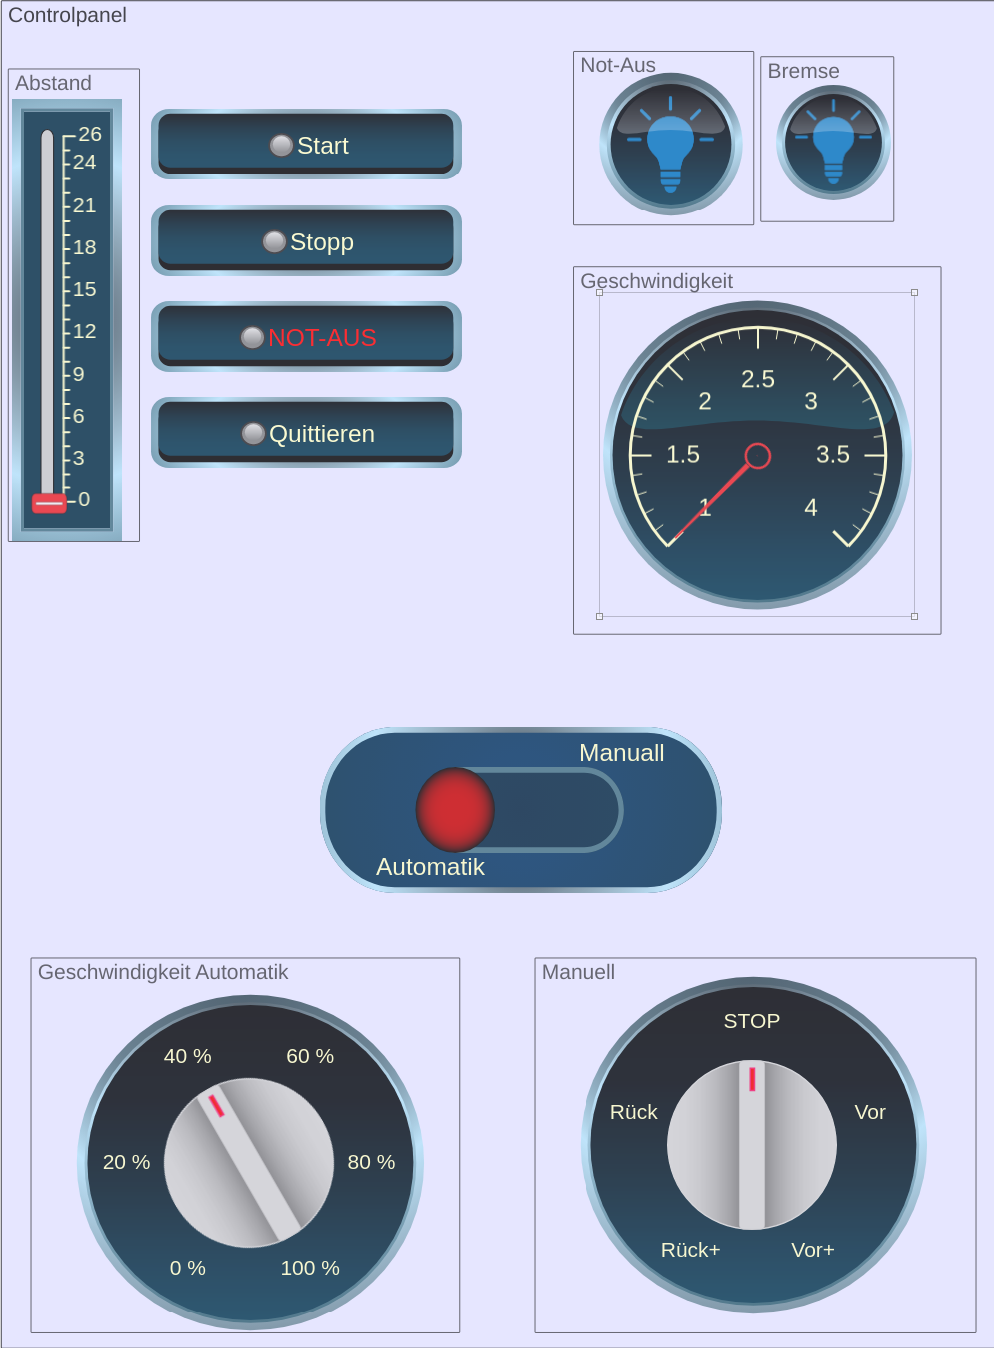
\includegraphics[width=\textwidth]{img/5_simulation/Automat_con.png}
		\caption{Automat – Controlpanel}
		\label{Controlpanel:img:Controlpanel}
	\end{center}
\end{figure}
\pagebreak[4]


\subsection{Automatensteuerung}
\label{Automatensteuerung}
Die Automatensteuerung beschreibt die logische Steuerung eines Systems durch einen Automaten, wie etwa einen Moore- oder Mealy-Automaten, der auf Basis von Eingaben und aktuellen Zuständen Ausgaben steuert.\\
Das Fahrzeug wird mittels eines Moore-Automaten gesteuert, wobei die Ausgänge erst dann aktiviert werden, wenn sich das System im entsprechenden Zustand befindet.\\ \ \\
Der Automat startet im Zustand \frqq Idle\flqq\ siehe Abbildung \ref{Automat_man:tab:z_idle}, und die Abläufe für den automatischen oder manuellen Modus werden von \frqq Idle\flqq\ aus angesteuert. Im Zustand Idle werden die Ausgänge (siehe Tabelle \ref{Automat_man:tab:z_idle}) geschaltet.\\

\pagebreak[1]
\begin{figure}[!ht]
	\begin{center}
		\includegraphics[width=0.75\textwidth]{img/5_simulation/Automat_idle.png}
		\caption{Automat – Start Zustand \frqq Idle\flqq}
		\label{Automat_man:img:start_idle}
	\end{center}
\end{figure}
\pagebreak[4]


\pagebreak[1]
\begin{table}[!ht]
	\centering
	\caption{Ausgänge – Idle}
	\label{Automat_man:tab:z_idle}
	\begin{tabular}{lll}
		\hline
		\textbf{Ausgänge}                           & \textbf{I/O Module}                 & \textbf{Wert} \\ \hline
		\multicolumn{1}{l|}{speed out}              & \multicolumn{1}{l|}{IO397-50k – A1} & 1             \\
		\multicolumn{1}{l|}{Driving(1)}             & \multicolumn{1}{l|}{}               & Reset         \\
		\multicolumn{1}{l|}{break motor out}        & \multicolumn{1}{l|}{IO397-50k – B3} & 5             \\
		\multicolumn{1}{l|}{direction out}          & \multicolumn{1}{l|}{IO397-50k – B4} & 5             \\
		\multicolumn{1}{l|}{cruise out}             & \multicolumn{1}{l|}{IO397-50k – B5} & 5             \\
		\multicolumn{1}{l|}{break mechanically out} & \multicolumn{1}{l|}{IO397-50k – B6} & 5             \\
		\multicolumn{1}{l|}{emergency stop out}     & \multicolumn{1}{l|}{IO397-50k – B7} & 0             \\ \hline
	\end{tabular}
\end{table}
\pagebreak[1]

Die Funktion \frqq Driving\flqq, siehe Abbildung \ref{Automat:img:fnc_Driving}, erhält einen Eingangswert, der durch einen \frqq Rate Limiter\flqq\ begrenzt und am Ausgang ausgegeben wird. Die Funktion speichert den letzten Wert, daher muss sie in den Zuständen, in denen das Fahrzeug angehalten wird, zurückgesetzt werden. Dies geschieht, indem die Funktion \frqq Driving\flqq\ den Wert \frqq 1\flqq\ erhält.\\

\pagebreak[1]
\begin{figure}[!ht]
	\begin{center}
		\includegraphics[width=.5\textwidth]{img/5_simulation/Automat_funktion_1.png}
		\includegraphics[width=.75\textwidth]{img/5_simulation/Automat_funktion_2.png}
		\caption{Automat – Funktion Driving}
		\label{Automat:img:fnc_Driving}
	\end{center}
\end{figure}
\pagebreak[4]

Der Zustand \frqq Emergency stop\flqq\ kann von jedem Zustand aus durch den Eingang \frqq emergency stop in\flqq\ erreicht werden, welcher sowohl über das Controlpanel als auch extern über das IO397-50k – B11 ausgelöst werden kann. Der Zustand kann nur durch die Quittierung verlassen werden und führt dann in einen der Idle-Zustände zurück: \frqq Idle\flqq\ \frqq Manual idle\flqq\ oder \frqq Automatic idle\flqq. Im Zustand \frqq Emergency stop\flqq\ werden die Ausgänge gemäß Tabelle \ref{Automat_man:tab:z_Emergency_stop} geschaltet.


\pagebreak[1]
\begin{table}[!ht]
	\centering
	\caption{Ausgänge – Emergency stop}
	\label{Automat_man:tab:z_Emergency_stop}
	\begin{tabular}{lll}
		\hline
		\textbf{Ausgänge}                           & \makecell{\textbf{I/O Module}         \\ \textbf{IO397-50k}}                 & \textbf{Wert} \\ \hline
		\multicolumn{1}{l|}{speed out=Driving()}    & \multicolumn{1}{l|}{A1}       & Reset \\
		\multicolumn{1}{l|}{break motor out}        & \multicolumn{1}{l|}{}         & 5     \\
		\multicolumn{1}{l|}{direction out}          & \multicolumn{1}{l|}{B4}       & 5     \\
		\multicolumn{1}{l|}{cruise out}             & \multicolumn{1}{l|}{B5}       & 5     \\
		\multicolumn{1}{l|}{break mechanically out} & \multicolumn{1}{l|}{B6}       & 5     \\
		\multicolumn{1}{l|}{emergency stop out}     & \multicolumn{1}{l|}{B7}       & 5     \\ \hline
	\end{tabular}
\end{table}
\pagebreak[1]










\subsubsection{Automat für die manuelle Steuerung}
\label{Automatensteuerung:Automat_man}

Die manuelle Steuerung bietet dem Nutzer die Flexibilität, das Fahrzeug sowohl innerhalb als auch außerhalb der Röhre zu steuern.\\

Der Automat des manuellen Ablaufs, wie in Abbildung \ref{Automat_man:img:man_übersicht} dargestellt, ist in zwei Stateflows unterteilt: \frqq Forwards\flqq\ und \frqq Backwards\flqq . In Abbildung \ref{Automat_man:img:man_vorwärts} ist der \frqq Forwards\flqq\ -Stateflow zu sehen, der \frqq Backwards\flqq\ -Stateflow ist äquivalent, wobei sich lediglich der Ausgang \frqq Direction Out\flqq\ ändert. Daher wird nur der \frqq Forwards\flqq\ -Stateflow erklärt. Der Zustand \frqq Emerency stop 1\flqq\ ist der gleiche Zustand wie \frqq Emergency stop\flqq.
Die Ausgänge für die Zustände \frqq Forwards\flqq\ und \frqq Backwards\flqq\ sind in 2 Tabellen aufgeführt \ref{Automat_man:tab:z_V_langsam} und \ref{Automat_man:tab:z_V_schnell} aufgeführt, hierbei ist die erste Tabelle die Zustände \frqq slow\flqq\ und die zweite Tabelle für die Zustände \frqq fast\flqq.





\pagebreak[1]
\begin{figure}[!ht]
	\begin{center}
		\includegraphics[width=0.9\textwidth]{img/5_simulation/Automat_man_uebersicht.png}
		\caption{Automat – Übersicht der manuellen Steuerung}
		\label{Automat_man:img:man_übersicht}
	\end{center}
\end{figure}
\pagebreak[1]


\pagebreak[1]
\begin{table}[!ht]
	\centering
	\caption{Ausgänge – der Zustände \frqq Forwards\flqq\ und \frqq Backwards\flqq\ –  \frqq slow\flqq}
	\label{Automat_man:tab:z_V_langsam}
	\begin{tabular}{llcc}
		\hline
		\textbf{Ausgänge}                             & \makecell{\textbf{I/O Module}             \\ \textbf{IO397-50k}}     & \makecell{\textbf{Werte}       \\ \textbf{\frqq Forwards\flqq}} & \makecell{\textbf{Werte}     \\ \textbf{\frqq Backwards\flqq}}  \\ \hline
		\multicolumn{1}{l|}{speed out=Driving$(1,5)$} & \multicolumn{1}{l|}{A1}       & 1,5 & 1,5 \\
		\multicolumn{1}{l|}{break motor out}          & \multicolumn{1}{l|}{B3}       & 1   & 1   \\
		\multicolumn{1}{l|}{direction out}            & \multicolumn{1}{l|}{B4}       & 5   & 0   \\
		\multicolumn{1}{l|}{cruise out}               & \multicolumn{1}{l|}{B5}       & 5   & 5   \\
		\multicolumn{1}{l|}{break mechanically out}   & \multicolumn{1}{l|}{B6}       & 0   & 0   \\
		\multicolumn{1}{l|}{emergency stop out}       & \multicolumn{1}{l|}{B7}       & 0   & 0   \\ \hline
	\end{tabular}
\end{table}
\pagebreak[1]

\pagebreak[1]
\begin{table}[!ht]
	\centering
	\caption{Ausgänge – der Zustände \frqq Forwards\flqq\ und \frqq Backwards\flqq\ –  \frqq fast\flqq}
	\label{Automat_man:tab:z_V_schnell}
	\begin{tabular}{cccc}
		\hline
		\textbf{Ausgänge}                           & \makecell{\textbf{I/O Module}         \\ \textbf{IO397-50k}}    & \makecell{\textbf{Werte}     \\ \textbf{\frqq Forwards\flqq}} & \makecell{\textbf{Werte}     \\ \textbf{\frqq Backwards\flqq}} \\ \hline
		\multicolumn{1}{l|}{speed out=Driving$(3)$} & \multicolumn{1}{l|}{A1}       & 3 & 3 \\
		\multicolumn{1}{l|}{break motor out}        & \multicolumn{1}{l|}{B3}       & 1 & 1 \\
		\multicolumn{1}{l|}{direction out}          & \multicolumn{1}{l|}{B4}       & 5 & 0 \\
		\multicolumn{1}{l|}{cruise out}             & \multicolumn{1}{l|}{B5}       & 5 & 5 \\
		\multicolumn{1}{l|}{break mechanically out} & \multicolumn{1}{l|}{B6}       & 0 & 0 \\
		\multicolumn{1}{l|}{emergency stop out}     & \multicolumn{1}{l|}{B7}       & 0 & 0 \\ \hline
	\end{tabular}
\end{table}
\pagebreak[1]

\pagebreak[1]
\begin{figure}[!ht]
	\begin{center}
		\includegraphics[width=\textwidth]{img/5_simulation/Automat_man_vorwaerts.png}
		\caption{Automat – \frqq Forwards\flqq\ -Stateflow der manuellen Steuerung}
		\label{Automat_man:img:man_vorwärts}
	\end{center}
\end{figure}
\pagebreak[1]



Mit dem Wahltaster (siehe Tabelle \ref{Controlpanel:tab:Wahlschalter}) kann zwischen den Zuständen gewechselt werden. In der Abbildung \ref{Automat_man:img:man_vorwärts} ist der Ausschnitt des \frqq Forwards\flqq\ -Stateflow zu sehen. Wenn sich der Automat in dem Stateflow \frqq Forwards\flqq\ befindet, gibt es keine direkte Verknüpfung zu dem \frqq Backwards\flqq\ Stateflow, somit muss man erst in den Zustand \frqq Manual idle\flqq\ wechseln, um in den Stateflow \frqq Backwards\flqq\ zu gelangen.

Der Zustand \frqq Collector manual in\flqq\ fängt  das Schaltsignal des Wahlschalters ab, wenn mitten im Betrieb auf Automatik geschalten wird und führt in dem \frqq Idle \flqq\ Zustand.









\subsubsection{Automat für die automatische Steuerung}
\label{Automatensteuerung:Automat_auto}


Die automatische Steuerung soll das Fahrzeug innerhalb der Röhre bis zur eingestellten Geschwindigkeit beschleunigen. Ab einer bestimmten Distanz zum Ende der Röhre soll es allmählich abbremsen und schließlich zum Stillstand kommen.

Der Automat \frqq Automatic\flqq\ besteht aus den Zuständen \frqq Automatic\flqq, \frqq Drive\flqq, \frqq Distance\flqq, \frqq Stop\flqq\ und \frqq Emergency stop\flqq, die in Abbildung \ref{Automat:img:auto_übersicht} dargestellt sind.\\
Der Zustand \frqq Automatic\flqq\ beschreibt den Idle-Zustand der automatischen Steuerung. Von hier aus wird der Zustand \frqq Drive\flqq\ angesteuert, sobald der Startknopf des \frqq Control Panels\flqq\ (siehe Abbildung \ref{Controlpanel:img:Controlpanel}) betätigt wird. Die Ausgänge werden gemäß Tabelle \ref{Automat_man:tab:automatic} gesetzt, solange der Zustand \frqq Automatic\flqq\ nicht verlassen wird.\\
Im Zustand \frqq Drive\flqq\ wird die Geschwindigkeit vom Nutzer mittels des Drehrads \frqq Geschwindigkeit Automatik\flqq\ eingestellt. Wird hingegen der \frqq Stop\flqq\ Taster betätigt, wird der Zustand \frqq Stop\flqq\ angesteuert. Ab einer Distanz von 10 m wird der Zustand \frqq Distance\flqq\ aktiviert. In Tabelle \ref{Automat_man:tab:drive} sind die Ausgänge des Zustands \frqq Drive\flqq\ dargestellt.\\
Wie bereits erwähnt, wird die Geschwindigkeit in Abhängigkeit vom Abstand \frqq distance\flqq\ zum Ende der Röhre verringert, hierbei wird in dem Zustand \frqq Distance\flqq\ der Augang der Geschwindigkeit mittels folgender Gleichung ermittelt:

\pagebreak[1]
\begin{align}
	\label{eq:speedout}
	speed_{out} = distance_{in}\cdot\frac{speed_{in}-1}{distance}+1
\end{align}
\pagebreak[1]

Soll die Automatik beendet werden, kann dies über den Stopp-Taster auf dem Control Panel ausgelöst werden. Dabei werden die in Tabelle \ref{Automat_man:tab:stop} aufgeführten Signale geschaltet.

\pagebreak[1]
\begin{table}[!ht]
	\centering
	\caption{Ausgänge – Automatic}
	\label{Automat_man:tab:automatic}
	\begin{tabular}{lll}
		\hline
		\textbf{Ausgänge}                           & \makecell{\textbf{I/O Module}             \\ \textbf{IO397-50k}}                 & \textbf{Wert} \\ \hline
		\multicolumn{1}{l|}{speed out}              & \multicolumn{1}{l|}{A1}       & Driving() \\
		\multicolumn{1}{l|}{Driving(1)}             & \multicolumn{1}{l|}{}         & Reset     \\
		\multicolumn{1}{l|}{break motor out}        & \multicolumn{1}{l|}{B3}       & 5         \\
		\multicolumn{1}{l|}{direction out}          & \multicolumn{1}{l|}{B4}       & 5         \\
		\multicolumn{1}{l|}{cruise out}             & \multicolumn{1}{l|}{B5}       & 5         \\
		\multicolumn{1}{l|}{break mechanically out} & \multicolumn{1}{l|}{B6}       & 5         \\
		\multicolumn{1}{l|}{emergency stop out}     & \multicolumn{1}{l|}{B7}       & 5         \\ \hline
	\end{tabular}
\end{table}
\pagebreak[2]



\pagebreak[1]
\begin{table}[!ht]
	\centering
	\caption{Ausgänge – Drive}
	\label{Automat_man:tab:drive}
	\begin{tabular}{lll}
		\hline
		\textbf{Ausgänge}                           & \makecell{\textbf{I/O Module}                     \\ \textbf{IO397-50k}}                 & \textbf{Wert} \\ \hline
		\multicolumn{1}{l|}{speed out}              & \multicolumn{1}{l|}{A1}       & Driving(speed in) \\
		\multicolumn{1}{l|}{Driving(speed in)}      & \multicolumn{1}{l|}{}         & speed in          \\
		\multicolumn{1}{l|}{break motor out}        & \multicolumn{1}{l|}{B3}       & 5                 \\
		\multicolumn{1}{l|}{direction out}          & \multicolumn{1}{l|}{B4}       & 5                 \\
		\multicolumn{1}{l|}{cruise out}             & \multicolumn{1}{l|}{B5}       & 5                 \\
		\multicolumn{1}{l|}{break mechanically out} & \multicolumn{1}{l|}{B6}       & 5                 \\
		\multicolumn{1}{l|}{emergency stop out}     & \multicolumn{1}{l|}{B7}       & 5                 \\ \hline
	\end{tabular}
\end{table}
\pagebreak[2]


\pagebreak[1]
\begin{table}[!ht]
	\centering
	\caption{Ausgänge – Distance}
	\label{Automat_man:tab:distance}
	\begin{tabular}{lll}
		\hline
		\textbf{Ausgänge}                           & \makecell{\textbf{I/O Module}                         \\ \textbf{IO397-50k}}                 & \textbf{Wert} \\ \hline
		\multicolumn{1}{l|}{speed out}              & \multicolumn{1}{l|}{A1}       & gl. \ref{eq:speedout} \\
		\multicolumn{1}{l|}{Driving(1)}             & \multicolumn{1}{l|}{}         & distance in           \\
		\multicolumn{1}{l|}{break motor out}        & \multicolumn{1}{l|}{B3}       & 1                     \\
		\multicolumn{1}{l|}{direction out}          & \multicolumn{1}{l|}{B4}       & 5                     \\
		\multicolumn{1}{l|}{cruise out}             & \multicolumn{1}{l|}{B5}       & 5                     \\
		\multicolumn{1}{l|}{break mechanically out} & \multicolumn{1}{l|}{B6}       & 0                     \\
		\multicolumn{1}{l|}{emergency stop out}     & \multicolumn{1}{l|}{B7}       & 0                     \\ \hline
	\end{tabular}
\end{table}
\pagebreak[2]


\pagebreak[1]
\begin{table}[!ht]
	\centering
	\caption{Ausgänge – Stop}
	\label{Automat_man:tab:stop}
	\begin{tabular}{lll}
		\hline
		\textbf{Ausgänge}                           & \makecell{\textbf{I/O Module}             \\ \textbf{IO397-50k}}                 & \textbf{Wert} \\ \hline
		\multicolumn{1}{l|}{speed out}              & \multicolumn{1}{l|}{A1}       & Driving() \\
		\multicolumn{1}{l|}{Driving(Reset)}         & \multicolumn{1}{l|}{}         & Reset     \\
		\multicolumn{1}{l|}{break motor out}        & \multicolumn{1}{l|}{B3}       & 1         \\
		\multicolumn{1}{l|}{direction out}          & \multicolumn{1}{l|}{B4}       & 5         \\
		\multicolumn{1}{l|}{cruise out}             & \multicolumn{1}{l|}{B5}       & 5         \\
		\multicolumn{1}{l|}{break mechanically out} & \multicolumn{1}{l|}{B6}       & 0         \\
		\multicolumn{1}{l|}{emergency stop out}     & \multicolumn{1}{l|}{B7}       & 0         \\ \hline
	\end{tabular}
\end{table}
\pagebreak[2]

\pagebreak[1]
\begin{figure}[!ht]
	\begin{center}
		\includegraphics[width=\textwidth]{img/5_simulation/Automat_auto_uebersicht.png}
		\caption{Automat – Übersicht der automatischen Steuerung}
		\label{Automat:img:auto_übersicht}
	\end{center}
\end{figure}
\pagebreak[4]
\
%%%%%%%%%%%%%%%%%%%%%%%%%%%%%%%%%%%%%%%%%%%%%%%%%%%%%%%%%%%%%%%%%%%%%%%%%%%%%%%%%%%%
%%%%%%%%%%%%%%%%%%%%%%%%%%%%%%%%%%%%%%%%%%%%%%%%%%%%%%%%%%%%%%%%%%%%%%%%%%%%%%%%%%%%
%%%%%%%%%%%%%%%%%%%%%%%%%%%%%%%%%%%%%%%%%%%%%%%%%%%%%%%%%%%%%%%%%%%%%%%%%%%%%%%%%%%%
%%%%%%%%%%%%%%%%%%%%%%%%%%%%%%%%%%%%%%%%%%%%%%%%%%%%%%%%%%%%%%%%%%%%%%%%%%%%%%%%%%%%
%%%%%%%%%%%%%%%%%%%%%%%%%%%%%%%%%%%%%%%%%%%%%%%%%%%%%%%%%%%%%%%%%%%%%%%%%%%%%%%%%%%%
%%%%%%%%%%%%%%%%%%%%%%%%%%%%%%%%%%%%%%%%%%%%%%%%%%%%%%%%%%%%%%%%%%%%%%%%%%%%%%%%%%%%

\newpage
\section{Distanzmessung}
\label{Distanzmessung}
%
%\myboxy{
%	\begin{itemize}
%		\item + Anschlüsse herauszufinden vier anschlüsse gefunden.
%		\item + Was für Aufgaben haben die Anschlüsse?
%		      \subitem Was für ein Kommunikationsprotokol hat der Sensor?
%		      \subitem Asynchron und seriell mit Baudrate 115200. (Ozilloskop)
%		\item mit einem ESP32 die Sensordaten lesen.
%		\item Nachrichtdekodierung (Controller MCU)
%		      \subitem Ox24 Start (Nachricht start)
%		      \subitem 0x26 Stopp (Nachricht ende)
%		      \subitem 24 30 30 30 33 32 36 30 30 32 39 26 (Stopp signal)
%		      \subitem 24 30 30 30 33 32 36 30 31 33 30 26 (Laser an)
%		      \subitem 24 30 30 30 32 32 31 32 33 26 (Messen)
%	\end{itemize}}{To-do}{\textwidth}
%
%

Ursprünglich wurde ein Sensor von Pepperl+Fuchs für die Distanzmessung angeschafft. Da dieser Sensor jedoch sehr teuer ist und wir nicht das Risiko eines möglichen Schadens im Vakuum eingehen wollten, wurde nach einer kostengünstigen Alternative gesucht.\\
Dafür wurde ein günstiges Entfernungsmessgerät für den Heimbedarf angeschafft und analysiert, ob es für die Anwendung geeignet ist.


\subsection{Verbindung}

Der Sensor ist über ein Flachbandkabel mit der Hauptplatine verbunden, wie in Abbildung \ref{img_2_2:sen_dis_parkside:1} zu sehen ist. Auf der Hauptplatine befinden sich vier ungenutzte Lötstellen. Mithilfe eines Oszilloskops und eines Multimeters wurden die Signale an den Lötstellen analysiert, wobei festgestellt wurde, dass Leitung \frqq 1\flqq\ eine Spannung von 3,3 V führt und Leitung \frqq 4\flqq\ als GND dient. Die Leitungen \frqq 2\flqq\ und \frqq 3\flqq\ übertragen digitale Signale und fungieren als Datenleitungen.

Die Kommunikation kann bei einer zweiadrigen Verbindung entweder synchron oder asynchron erfolgen. Bei synchroner Kommunikation dient eine der Leitungen als Taktleitung (Clock). Bei asynchroner Kommunikation ist eine Leitung der Sender (TX) und die andere der Empfänger (RX). Zur Überprüfung der Kommunikationsart wurde ein Oszillogramm (siehe Abbildung \ref{parkside:ozi:datenübertragung}) aufgenommen. Im Oszillogramm wurde kein Taktsignal festgestellt, sodass die Datenübertragung asynchron und Vollduplex erfolgt. In Tabelle \ref{parkside:pinmapping} ist die Pinbelegung aufgelistet.\\



\pagebreak[1]
\begin{figure}[!ht]
	\begin{center}
		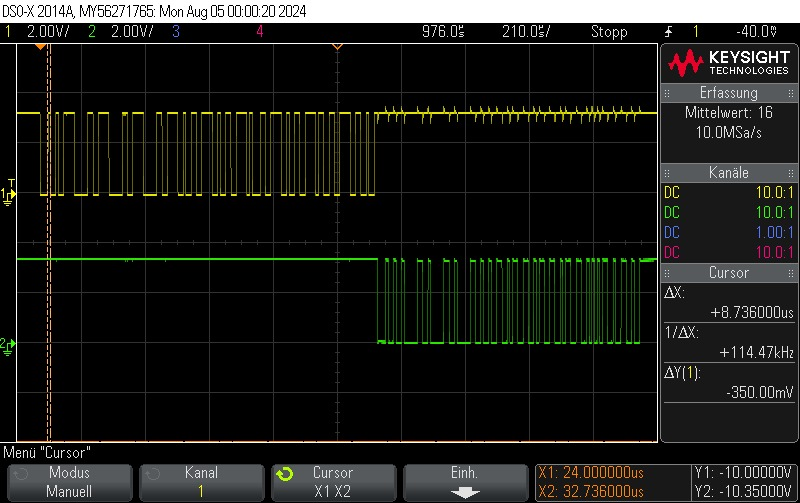
\includegraphics[width=\textwidth]{img/2_sen/ozi_3.png}
		\caption{Messung – zur Überprüfung der Kommunikationsart: Synchron oder Asynchron}
		\label{parkside:ozi:datenübertragung}
	\end{center}
\end{figure}
\pagebreak[1]




\pagebreak[1]
\begin{table}[!ht]
	\centering
	\caption{PARKSIDE – Pin Mapping – Distanzsensor}
	\label{parkside:pinmapping}
	\begin{tabular}{l|ll}
		\hline
		\textbf{Pin} & \textbf{Farbe} & \textbf{Funktion} \\ \hline
		1            & Rot            & 3V3               \\
		2            & Weiß           & RX (receiver)     \\
		3            & Gelb           & TX (transmitter)  \\
		4            & Schwarz        & GND               \\ \hline
	\end{tabular}
\end{table}
\pagebreak[1]

\pagebreak[1]
\begin{figure}[!ht]
	\begin{center}
		\includegraphics[width=1\textwidth]{img/2_sen/dis_parkside_1_outside.png}
		\caption{PARKSIDE – Distanzsensor – Innenaufbau}
		\label{img_2_2:sen_dis_parkside:1}
	\end{center}
\end{figure}
\pagebreak[4]

\subsection{Dekodierung der Steuersignale}
\label{Distanzmessung:Kodierung}
Um die Steuersignale zu analysieren, wurden die mit dem Oszilloskop aufgenommenen Messwerte in den Tabellen \ref{Steuerung:tab:TX1}, \ref{Steuerung:tab:RX1} und \ref{Steuerung:tab:RX2} dokumentiert. Bei den Messungen fiel auf, dass jede Nachricht mit dem Bitmuster \frqq 0x24\flqq\ (Nachricht-Start) beginnt und mit dem Bitmuster \frqq 0x26\flqq\ (Nachricht-Ende) endet. Zwischen diesen beiden Bitmustern sind die Steuersignale und Messwerte kodiert, welche im Folgenden erklärt werden.\\
\
\pagebreak[1]
\begin{figure}[!ht]
	\begin{center}
		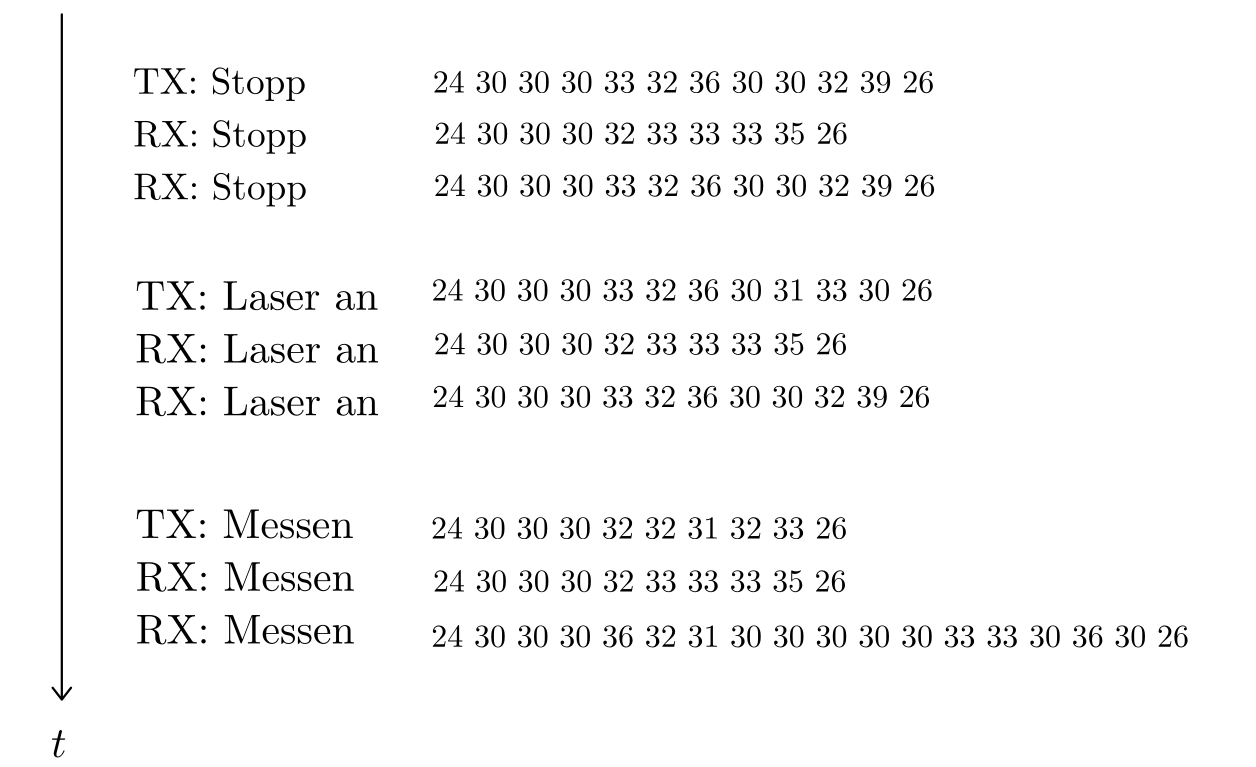
\includegraphics[width=1\textwidth]{img/2_sen/dis_parkside_signalverlauf.png}
		\caption{Distanzmessung – Signalverlauf der Steuersignale}
		\label{Kodierung:pic:signalverlauf}
	\end{center}
\end{figure}
\pagebreak[4]
Die Signalübertragung in den Tabellen ist wie folgt aufgebaut: In Tabelle \ref{Steuerung:tab:TX1} zeigt die Spalte \frqq Stopp\flqq\ die erste Nachricht, die an den Sensor gesendet wird. Der Sensor antwortet stets mit zwei Nachrichten: Die erste Nachricht ist in Tabelle \ref{Steuerung:tab:RX1} dargestellt, die zweite in Tabelle \ref{Steuerung:tab:RX2}, in der Abbildung \ref{Kodierung:pic:signalverlauf} ist der Verlauf noch einmal aufgeführt.\\ \ \\
Die gelb hinterlegten Felder in den Tabellen weisen auf ein identisches Bitmuster hin. Nach jedem Start-Byte werden drei identisch kodierte Bytes gesendet, die als Delay fungieren. Der Sensor antwortet nach jedem \frqq Transmitter\flqq\ Signal mit derselben Kodierung, was als Bestätigung dient, dass er sendebereit ist. Erst wenn das Bitmuster \frqq Messen\flqq\ an den Sensor gesendet wird, überträgt der Sensor die Messdaten, die in den grün hinterlegten Feldern in Tabelle \ref{Steuerung:tab:RX2} als ASCII-Zeichen dargestellt sind.


\pagebreak[4]
\begin{table}[!ht]
	\centering
	\caption{Distanzmessung – Signale die an den Sensor gesendet werden (TX)}
	\label{Steuerung:tab:TX1}
	\begin{tabular}{lllllll}
		\hline
		                        & \multicolumn{2}{c}{TX Stopp} & \multicolumn{2}{c}{ TX Laser an}                   & \multicolumn{2}{c}{TX Messen}                                                                                                                   \\ \hline
		\textbf{Bytes}          & \textbf{Nachricht}           & \textbf{Bdtg.}                                     & \textbf{Nachricht}            & \textbf{Bdtg.}                                     & \textbf{Nachricht}         & \textbf{Bdtg.}                \\ \hline
		\multicolumn{1}{l|}{0}  & \cellcolor[HTML]{9AFF99}24   & \multicolumn{1}{l|}{\cellcolor[HTML]{9AFF99}Start} & \cellcolor[HTML]{9AFF99}24    & \multicolumn{1}{l|}{\cellcolor[HTML]{9AFF99}Start} & \cellcolor[HTML]{9AFF99}24 & \cellcolor[HTML]{9AFF99}Start \\
		\multicolumn{1}{l|}{1}  & \cellcolor[HTML]{FCFF2F}30   & \multicolumn{1}{l|}{\cellcolor[HTML]{FCFF2F}}      & \cellcolor[HTML]{FCFF2F}30    & \multicolumn{1}{l|}{\cellcolor[HTML]{FCFF2F}}      & \cellcolor[HTML]{FCFF2F}30 & \cellcolor[HTML]{FCFF2F}      \\
		\multicolumn{1}{l|}{2}  & \cellcolor[HTML]{FCFF2F}30   & \multicolumn{1}{l|}{\cellcolor[HTML]{FCFF2F}}      & \cellcolor[HTML]{FCFF2F}30    & \multicolumn{1}{l|}{\cellcolor[HTML]{FCFF2F}}      & \cellcolor[HTML]{FCFF2F}30 & \cellcolor[HTML]{FCFF2F}      \\
		\multicolumn{1}{l|}{3}  & \cellcolor[HTML]{FCFF2F}30   & \multicolumn{1}{l|}{\cellcolor[HTML]{FCFF2F}}      & \cellcolor[HTML]{FCFF2F}30    & \multicolumn{1}{l|}{\cellcolor[HTML]{FCFF2F}}      & \cellcolor[HTML]{FCFF2F}30 & \cellcolor[HTML]{FCFF2F}      \\
		\multicolumn{1}{l|}{4}  & 33                           & \multicolumn{1}{l|}{}                              & 33                            & \multicolumn{1}{l|}{}                              & 32                         &                               \\
		\multicolumn{1}{l|}{5}  & 32                           & \multicolumn{1}{l|}{}                              & 32                            & \multicolumn{1}{l|}{}                              & 32                         &                               \\
		\multicolumn{1}{l|}{6}  & 36                           & \multicolumn{1}{l|}{}                              & 36                            & \multicolumn{1}{l|}{}                              & 31                         &                               \\
		\multicolumn{1}{l|}{7}  & 30                           & \multicolumn{1}{l|}{}                              & 30                            & \multicolumn{1}{l|}{}                              & 32                         &                               \\
		\multicolumn{1}{l|}{8}  & 30                           & \multicolumn{1}{l|}{}                              & 31                            & \multicolumn{1}{l|}{}                              & 33                         &                               \\
		\multicolumn{1}{l|}{9}  & 32                           & \multicolumn{1}{l|}{}                              & 33                            & \multicolumn{1}{l|}{}                              & \cellcolor[HTML]{FD6864}26 & \cellcolor[HTML]{FD6864}Stop  \\
		\multicolumn{1}{l|}{10} & 39                           & \multicolumn{1}{l|}{}                              & 30                            & \multicolumn{1}{l|}{}                              &                            &                               \\
		\multicolumn{1}{l|}{11} & \cellcolor[HTML]{FD6864}26   & \multicolumn{1}{l|}{\cellcolor[HTML]{FD6864}Stop}  & \cellcolor[HTML]{FD6864}26    & \multicolumn{1}{l|}{\cellcolor[HTML]{FD6864}Stop}  &                            &                               \\ \hline
	\end{tabular}
\end{table}


\pagebreak[1]
\begin{table}[!ht]
	\centering
	\caption{Distanzmessung – Signale die von dem Sensor gesendet werden 1 (RX)}
	\label{Steuerung:tab:RX1}
	\begin{tabular}{lllllll}
		\hline
		                        & \multicolumn{2}{c}{RX Stopp} & \multicolumn{2}{c}{RX Laser an}                    & \multicolumn{2}{c}{RX Messen}                                                                                                                   \\ \hline
		\textbf{Bytes}          & \textbf{Nachricht}           & \textbf{Bdtg.}                                     & \textbf{Nachricht}            & \textbf{Bdtg.}                                     & \textbf{Nachricht}         & \textbf{Bdtg.}                \\ \hline
		\multicolumn{1}{l|}{0}  & \cellcolor[HTML]{9AFF99}24   & \multicolumn{1}{l|}{\cellcolor[HTML]{9AFF99}Start} & \cellcolor[HTML]{9AFF99}24    & \multicolumn{1}{l|}{\cellcolor[HTML]{9AFF99}Start} & \cellcolor[HTML]{9AFF99}24 & \cellcolor[HTML]{9AFF99}Start \\
		\multicolumn{1}{l|}{1}  & \cellcolor[HTML]{F8FF00}30   & \multicolumn{1}{l|}{\cellcolor[HTML]{F8FF00}}      & \cellcolor[HTML]{F8FF00}30    & \multicolumn{1}{l|}{\cellcolor[HTML]{F8FF00}}      & \cellcolor[HTML]{F8FF00}30 & \cellcolor[HTML]{F8FF00}      \\
		\multicolumn{1}{l|}{2}  & \cellcolor[HTML]{F8FF00}30   & \multicolumn{1}{l|}{\cellcolor[HTML]{F8FF00}}      & \cellcolor[HTML]{F8FF00}30    & \multicolumn{1}{l|}{\cellcolor[HTML]{F8FF00}}      & \cellcolor[HTML]{F8FF00}30 & \cellcolor[HTML]{F8FF00}      \\
		\multicolumn{1}{l|}{3}  & \cellcolor[HTML]{F8FF00}30   & \multicolumn{1}{l|}{\cellcolor[HTML]{F8FF00}}      & \cellcolor[HTML]{F8FF00}30    & \multicolumn{1}{l|}{\cellcolor[HTML]{F8FF00}}      & \cellcolor[HTML]{F8FF00}30 & \cellcolor[HTML]{F8FF00}      \\
		\multicolumn{1}{l|}{4}  & \cellcolor[HTML]{F8FF00}32   & \multicolumn{1}{l|}{\cellcolor[HTML]{F8FF00}}      & \cellcolor[HTML]{F8FF00}32    & \multicolumn{1}{l|}{\cellcolor[HTML]{F8FF00}}      & \cellcolor[HTML]{F8FF00}32 & \cellcolor[HTML]{F8FF00}      \\
		\multicolumn{1}{l|}{5}  & \cellcolor[HTML]{F8FF00}33   & \multicolumn{1}{l|}{\cellcolor[HTML]{F8FF00}}      & \cellcolor[HTML]{F8FF00}33    & \multicolumn{1}{l|}{\cellcolor[HTML]{F8FF00}}      & \cellcolor[HTML]{F8FF00}33 & \cellcolor[HTML]{F8FF00}      \\
		\multicolumn{1}{l|}{6}  & \cellcolor[HTML]{F8FF00}33   & \multicolumn{1}{l|}{\cellcolor[HTML]{F8FF00}}      & \cellcolor[HTML]{F8FF00}33    & \multicolumn{1}{l|}{\cellcolor[HTML]{F8FF00}}      & \cellcolor[HTML]{F8FF00}33 & \cellcolor[HTML]{F8FF00}      \\
		\multicolumn{1}{l|}{7}  & \cellcolor[HTML]{F8FF00}33   & \multicolumn{1}{l|}{\cellcolor[HTML]{F8FF00}}      & \cellcolor[HTML]{F8FF00}33    & \multicolumn{1}{l|}{\cellcolor[HTML]{F8FF00}}      & \cellcolor[HTML]{F8FF00}33 & \cellcolor[HTML]{F8FF00}      \\
		\multicolumn{1}{l|}{8}  & \cellcolor[HTML]{F8FF00}35   & \multicolumn{1}{l|}{\cellcolor[HTML]{F8FF00}}      & \cellcolor[HTML]{F8FF00}35    & \multicolumn{1}{l|}{\cellcolor[HTML]{F8FF00}}      & \cellcolor[HTML]{F8FF00}35 & \cellcolor[HTML]{F8FF00}      \\
		\multicolumn{1}{l|}{9}  & \cellcolor[HTML]{FD6864}26   & \multicolumn{1}{l|}{\cellcolor[HTML]{FD6864}Stop}  & \cellcolor[HTML]{FD6864}26    & \multicolumn{1}{l|}{\cellcolor[HTML]{FD6864}Stop}  & \cellcolor[HTML]{FD6864}26 & \cellcolor[HTML]{FD6864}Stop  \\
		\multicolumn{1}{l|}{10} &                              & \multicolumn{1}{l|}{}                              &                               & \multicolumn{1}{l|}{}                              &                            &                               \\
		\multicolumn{1}{l|}{11} &                              & \multicolumn{1}{l|}{}                              &                               & \multicolumn{1}{l|}{}                              &                            &                               \\ \hline
	\end{tabular}
\end{table}
\pagebreak[1]

\pagebreak[1]
\begin{table}[!ht]
	\centering
	\caption{Distanzmessung – Signale die von dem Sensor gesendet werden 2 (RX)}
	\label{Steuerung:tab:RX2}
	\begin{tabular}{lllllll}
		\hline
		                        & \multicolumn{2}{c}{RX Stopp} & \multicolumn{2}{c}{RX Laser an}                    & \multicolumn{2}{c}{RX Messen}                                                                                                                                    \\ \hline
		\textbf{Bytes}          & \textbf{Nachricht}           & \textbf{Bdtg.}                                     & \textbf{Nachricht}            & \textbf{Bdtg.}                                     & \textbf{Nachricht}         & \textbf{Bdtg.}                                 \\ \hline
		\multicolumn{1}{l|}{0}  & \cellcolor[HTML]{9AFF99}24   & \multicolumn{1}{l|}{\cellcolor[HTML]{9AFF99}Start} & \cellcolor[HTML]{9AFF99}24    & \multicolumn{1}{l|}{\cellcolor[HTML]{9AFF99}Start} & \cellcolor[HTML]{9AFF99}24 & \cellcolor[HTML]{9AFF99}Start                  \\
		\multicolumn{1}{l|}{1}  & \cellcolor[HTML]{F8FF00}30   & \multicolumn{1}{l|}{\cellcolor[HTML]{F8FF00}}      & \cellcolor[HTML]{F8FF00}30    & \multicolumn{1}{l|}{\cellcolor[HTML]{F8FF00}}      & \cellcolor[HTML]{F8FF00}30 & \cellcolor[HTML]{F8FF00}                       \\
		\multicolumn{1}{l|}{2}  & \cellcolor[HTML]{F8FF00}30   & \multicolumn{1}{l|}{\cellcolor[HTML]{F8FF00}}      & \cellcolor[HTML]{F8FF00}30    & \multicolumn{1}{l|}{\cellcolor[HTML]{F8FF00}}      & \cellcolor[HTML]{F8FF00}30 & \cellcolor[HTML]{F8FF00}                       \\
		\multicolumn{1}{l|}{3}  & \cellcolor[HTML]{F8FF00}30   & \multicolumn{1}{l|}{\cellcolor[HTML]{F8FF00}}      & \cellcolor[HTML]{F8FF00}30    & \multicolumn{1}{l|}{\cellcolor[HTML]{F8FF00}}      & \cellcolor[HTML]{F8FF00}30 & \cellcolor[HTML]{F8FF00}                       \\
		\multicolumn{1}{l|}{4}  & 33                           & \multicolumn{1}{l|}{}                              & 33                            & \multicolumn{1}{l|}{}                              & \cellcolor[HTML]{FFCC67}36 &                                                \\
		\multicolumn{1}{l|}{5}  & 32                           & \multicolumn{1}{l|}{}                              & 32                            & \multicolumn{1}{l|}{}                              & \cellcolor[HTML]{FFCC67}32 &                                                \\
		\multicolumn{1}{l|}{6}  & 36                           & \multicolumn{1}{l|}{}                              & 36                            & \multicolumn{1}{l|}{}                              & \cellcolor[HTML]{FFCC67}31 &                                                \\
		\multicolumn{1}{l|}{7}  & 30                           & \multicolumn{1}{l|}{}                              & 30                            & \multicolumn{1}{l|}{}                              & \cellcolor[HTML]{32CB00}30 & \cellcolor[HTML]{32CB00}10\textasciicircum{}+4 \\
		\multicolumn{1}{l|}{8}  & 30                           & \multicolumn{1}{l|}{}                              & 30                            & \multicolumn{1}{l|}{}                              & \cellcolor[HTML]{32CB00}30 & \cellcolor[HTML]{32CB00}10\textasciicircum{}+3 \\
		\multicolumn{1}{l|}{9}  & 32                           & \multicolumn{1}{l|}{}                              & 32                            & \multicolumn{1}{l|}{}                              & \cellcolor[HTML]{32CB00}30 & \cellcolor[HTML]{32CB00}10\textasciicircum{}+2 \\
		\multicolumn{1}{l|}{10} & 39                           & \multicolumn{1}{l|}{}                              & 39                            & \multicolumn{1}{l|}{}                              & \cellcolor[HTML]{32CB00}30 & \cellcolor[HTML]{32CB00}10\textasciicircum{}+1 \\
		\multicolumn{1}{l|}{11} & \cellcolor[HTML]{FD6864}26   & \multicolumn{1}{l|}{\cellcolor[HTML]{FD6864}Stop}  & \cellcolor[HTML]{FD6864}26    & \multicolumn{1}{l|}{\cellcolor[HTML]{FD6864}Stop}  & \cellcolor[HTML]{32CB00}30 & \cellcolor[HTML]{32CB00}10\textasciicircum{}+0 \\
		\multicolumn{1}{l|}{12} &                              & \multicolumn{1}{l|}{}                              &                               & \multicolumn{1}{l|}{}                              & \cellcolor[HTML]{32CB00}33 & \cellcolor[HTML]{32CB00}10\textasciicircum{}-1 \\
		\multicolumn{1}{l|}{13} &                              & \multicolumn{1}{l|}{}                              &                               & \multicolumn{1}{l|}{}                              & \cellcolor[HTML]{32CB00}33 & \cellcolor[HTML]{32CB00}10\textasciicircum{}-2 \\
		\multicolumn{1}{l|}{14} &                              & \multicolumn{1}{l|}{}                              &                               & \multicolumn{1}{l|}{}                              & \cellcolor[HTML]{32CB00}30 & \cellcolor[HTML]{32CB00}10\textasciicircum{}-3 \\
		\multicolumn{1}{l|}{15} &                              & \multicolumn{1}{l|}{}                              &                               & \multicolumn{1}{l|}{}                              & \cellcolor[HTML]{32CB00}36 & \cellcolor[HTML]{32CB00}10\textasciicircum{}-4 \\
		\multicolumn{1}{l|}{16} &                              & \multicolumn{1}{l|}{}                              &                               & \multicolumn{1}{l|}{}                              & \cellcolor[HTML]{32CB00}30 & \cellcolor[HTML]{32CB00}10\textasciicircum{}-5 \\
		\multicolumn{1}{l|}{17} &                              & \multicolumn{1}{l|}{}                              &                               & \multicolumn{1}{l|}{}                              & \cellcolor[HTML]{FD6864}26 & \cellcolor[HTML]{FD6864}Stop                   \\ \hline
	\end{tabular}
\end{table}
\pagebreak[4]

%\subsection{Steuerung für die Sensordaten}
%\label{Distanzmessung:Steuerung}
%
%
%Um die Werte von dem Distanzsensor zu erhalten wird eine ESP verwendet.




%%%%%%%%%%%%%%%%%%%%%%%%%%%%%%%%%%%%%%%%%%%%%%%%%%%%%%%%%%%%%%%%%%%%%%%%%%%%%%%%%%%%
%%%%%%%%%%%%%%%%%%%%%%%%%%%%%%%%%%%%%%%%%%%%%%%%%%%%%%%%%%%%%%%%%%%%%%%%%%%%%%%%%%%%
%%%%%%%%%%%%%%%%%%%%%%%%%%%%%%%%%%%%%%%%%%%%%%%%%%%%%%%%%%%%%%%%%%%%%%%%%%%%%%%%%%%%
%%%%%%%%%%%%%%%%%%%%%%%%%%%%%%%%%%%%%%%%%%%%%%%%%%%%%%%%%%%%%%%%%%%%%%%%%%%%%%%%%%%%
%%%%%%%%%%%%%%%%%%%%%%%%%%%%%%%%%%%%%%%%%%%%%%%%%%%%%%%%%%%%%%%%%%%%%%%%%%%%%%%%%%%%
%%%%%%%%%%%%%%%%%%%%%%%%%%%%%%%%%%%%%%%%%%%%%%%%%%%%%%%%%%%%%%%%%%%%%%%%%%%%%%%%%%%%


\include{source/einennoch}
\chapter{Konklusion}


In dieser Projektarbeit wurde erfolgreich ein funktionsfähiges Fahrzeug für den Hyperloop-Prototyp entwickelt und dessen Aufbau sowie die Steuerung detailliert beschrieben. Die Implementierung umfasste mehrere wesentliche Schritte: Von der Erstellung eines Schaltplans für die elektrische Verdrahtung über die Integration der Sensorik bis hin zur Programmierung und Simulation der Steuerungslogik.

Die Implementierung der Steuerung erfolgte über ein Speedgoat-System, das Echtzeitsteuerung ermöglicht. Die Simulation der Steuerungslogik in Simulink stellte sicher, dass das Fahrzeug sowohl im manuellen als auch im automatischen Modus betrieben werden kann. Im manuellen Modus kann der Benutzer das Fahrzeug vorwärts und rückwärts fahren lassen, während der automatische Modus das Fahrzeug beschleunigt und bei Annäherung an das Streckenende abbremst. Zudem wurde die Distanzmessung durch einen alternativen Sensor kostengünstig und zuverlässig realisiert, was die Positionierung des Fahrzeugs in der Röhre ermöglicht.

Die Wahl der Bauteile, wie des BLDC-Motors und der IO-Module, sowie die Verdrahtungskonventionen wurden sorgfältig dokumentiert und implementiert, um eine sichere und stabile Betriebsumgebung zu gewährleisten. Die entwickelten Endschnittstellen bieten eine Grundlage für zukünftige Erweiterungen und Testdurchläufe.

Zukünftige Arbeiten könnten darauf abzielen, das Fahrzeug unter realistischen Bedingungen zu testen, um das Zusammenspiel von Steuerung und Sensorik weiter zu optimieren. Die durchgeführten Implementierungen und die offene Architektur des Systems bieten somit eine flexible Basis für die Weiterentwicklung des Hyperloop-Konzepts und die Erforschung einer innovativen, energieeffizienten Transportlösung.
\include{source/einennoch}
\include{source/Literaturverzeichnis}
\printbibliography
\appendix
\include{source/einennoch}
\chapter{Anhang}
\section{Schaltplan}
\label{Anhang:Schaltplan}

\myboxy{
	\begin{itemize}
		\item BMK beschriftung anpassen
		\item Bauteile einpflegen
	\end{itemize}
}{To-do}{\textwidth}

%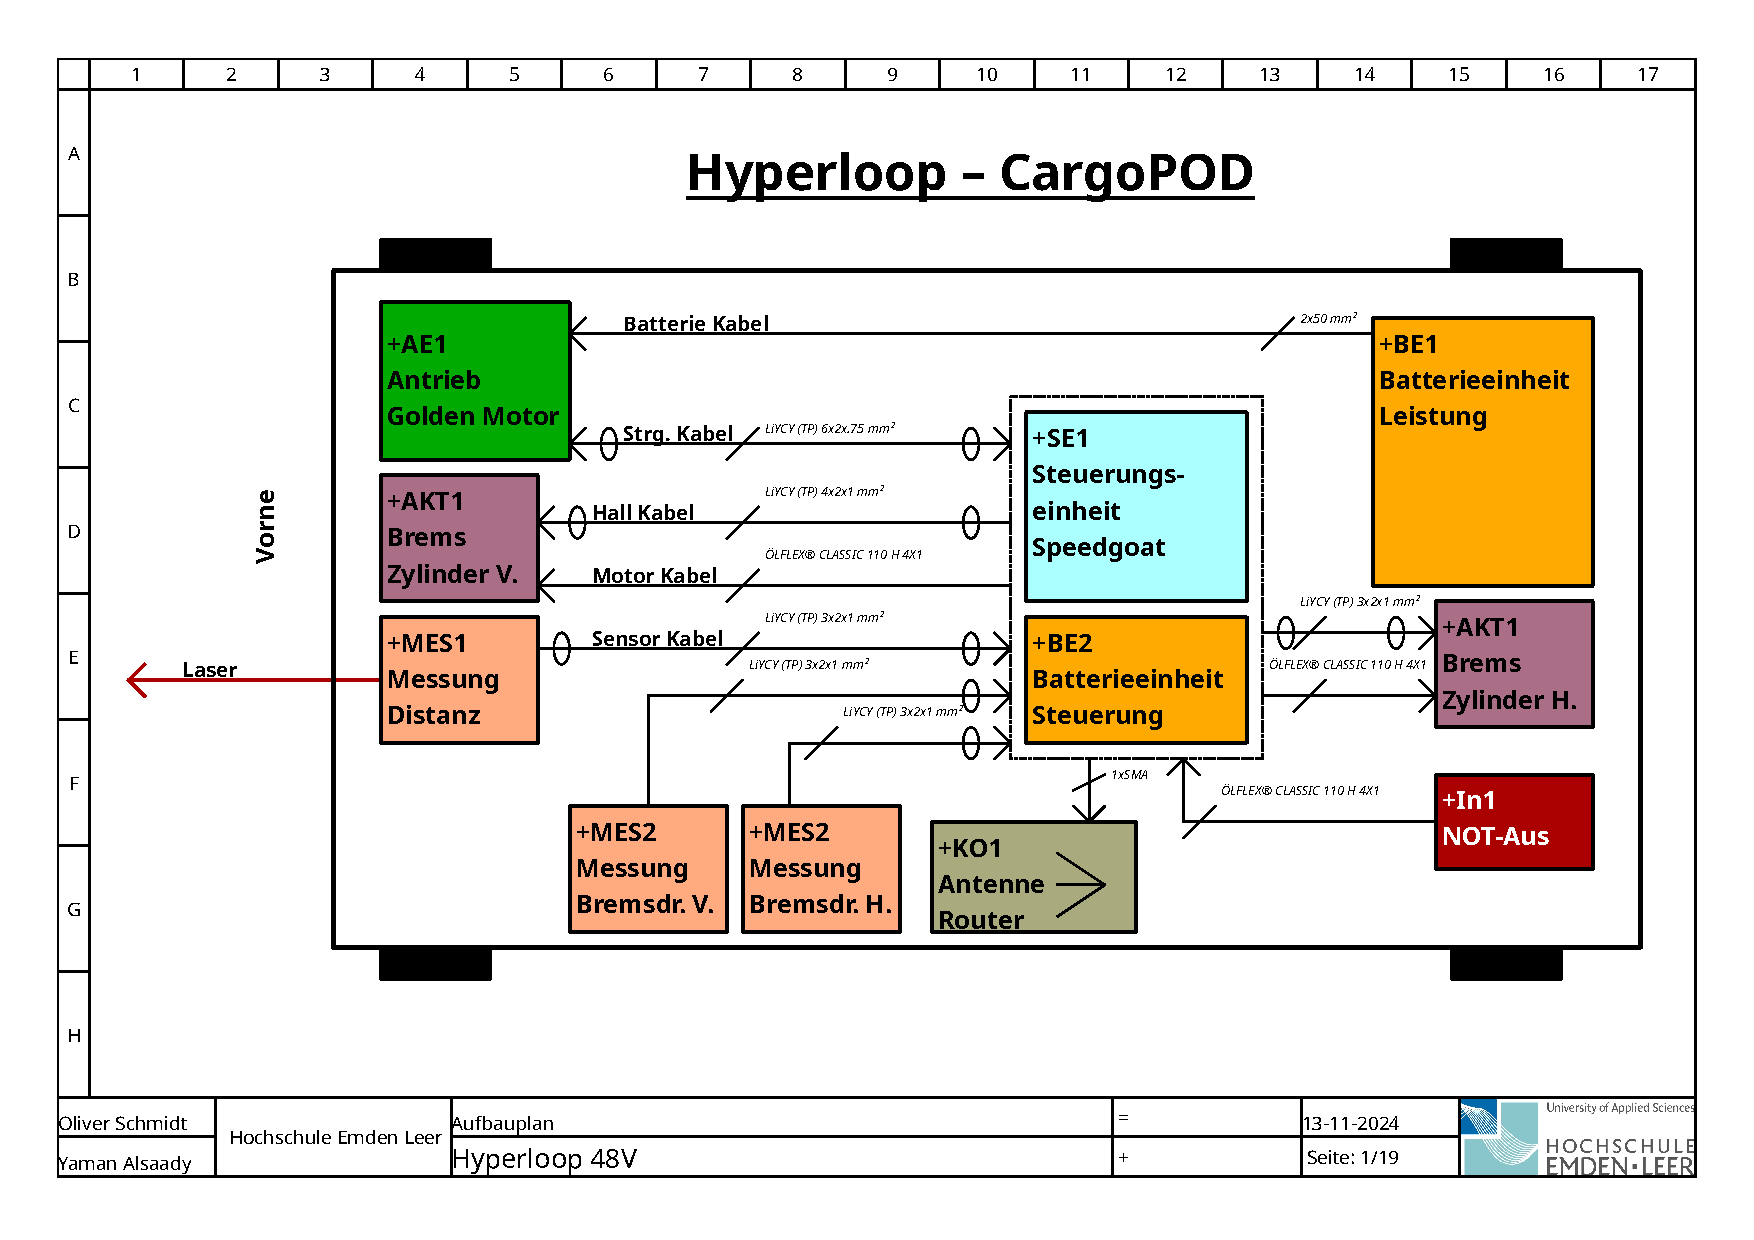
\includepdf[pages=-,landscape] {anhang/Schaltplan.pdf}


\end{document}
